\documentclass{article}
\usepackage[margin=1in]{geometry}
\usepackage{graphicx}
\usepackage[hidelinks]{hyperref}
\usepackage{xcolor}
\usepackage{listings}
\usepackage{inconsolata}
\usepackage{setspace}
\usepackage{parskip}
\usepackage{tikz}
\usepackage{textcomp}
\usepackage{fontspec}
\usepackage[many]{tcolorbox}
\usepackage{amsmath}
\usepackage{amssymb}
\usepackage{tcolorbox}
\usepackage{float}
\usetikzlibrary{shapes.multipart}

\usetikzlibrary{shapes.geometric, arrows.meta, matrix, positioning}
\setstretch{1.1}
\setlength{\parindent}{0pt}
\setmonofont{Courier New}[Scale=MatchLowercase]

\definecolor{codekw}{rgb}{0.15, 0.15, 0.15}
\definecolor{codestr}{rgb}{0.20, 0.40, 0.30}
\definecolor{codecmt}{rgb}{0.55, 0.55, 0.55}
\definecolor{codenum}{rgb}{0.40, 0.40, 0.40}
\definecolor{frameline}{rgb}{0.80, 0.80, 0.80}

\newtcolorbox{mdquote}{
    colback=gray!5,
    colframe=gray!40, 
    arc=0pt,
    outer arc=0pt,
    leftrule=4pt,
    rightrule=0pt,
    toprule=0pt,
    bottomrule=0pt,
    boxsep=0pt,
    left=10pt,
    right=10pt,
    top=8pt,
    bottom=8pt
}

\lstdefinestyle{python}{
    language=Python,
    basicstyle=\ttfamily\small\color{black!85},
    keywordstyle=\color{codekw}\bfseries,
    commentstyle=\color{codecmt}\itshape,
    stringstyle=\color{codestr},
    numberstyle=\ttfamily\tiny\color{codenum},
    numbers=left,
    stepnumber=1,
    numbersep=12pt,
    showstringspaces=false,
    tabsize=4,
    breaklines=true,
    keepspaces=true,
    columns=fixed,
    frame=tb,
    framerule=0.5pt,
    rulecolor=\color{frameline},
    framextopmargin=4pt,
    framexbottommargin=4pt,
    xleftmargin=18pt,
    framexleftmargin=0pt,
}

\newcounter{qcounter}

\newtcolorbox[use counter=qcounter]{Question}[2][]{
    enhanced,
    breakable,
    colback=white, 
    frame hidden,
    borderline north={0.5pt}{0pt}{frameline},
    borderline south={0.5pt}{0pt}{frameline},
    sharp corners,
    boxsep=0pt,
    left=0pt, right=0pt,
    top=10pt, bottom=10pt,
    before upper={\noindent\textbf{Q\thetcbcounter\ (#2).}\par\vspace{0.5em}},
    #1
}

\title{\Huge{\textsc{A Brief Cookbook of Coding}}}
\author{}
\date{}

\begin{document}

\maketitle

\tableofcontents

\vspace{4ex}

\emph{Do you know why the table of contents can't be part of the table of contents? Because of self-reference! And that's pretty much the core idea behind this coding cookbook.}

\newpage

\section*{}

\emph{For a better coding experience --- let’s use Python in this cookbook. This isn’t to criticize C++ or Java, but Python code is usually much easier to express ideas (while still offering good performance for most cases). We do not delve into low-level implementations in depth, as they are less important than their use within higher-level ideas.}

\emph{I used to code primarily in C++. Note that data structures and algorithms are far more important than any specific programming language. Try solving problems on \href{https://codeforces.com/}{Codeforces}, \href{https://leetcode.com/}{LeetCode} or \href{https://www.luogu.com.cn/}{Luogu} --- or any coding platform you prefer!}

\begin{flushright}
    \emph{rainrzk} \\
    \emph{Aug 2, 2026}
\end{flushright}


\newpage

\section{Data Structures}

\subsection{Linear Structures}

\subsubsection{Hashtable}

\textbf{Hashtable} is the \emph{first} linear structure I'm going to talk about.
We simply use

\begin{lstlisting}[style=python]
m = {}
\end{lstlisting}

to create a \emph{map / dict}.

A hashing process is defined by a function that maps a key to the index where its value is stored. In the best case, the time complexity is $\mathcal O(1)$.

\vspace{2em}

\begin{center}
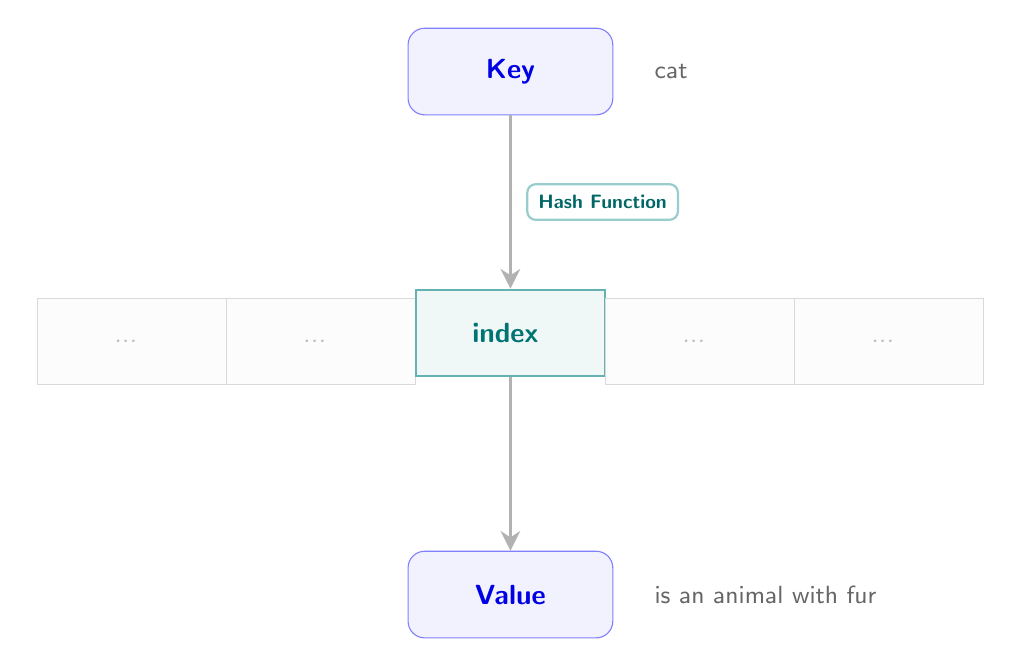
\begin{tikzpicture}[
    >={Stealth[length=2.5mm, width=2.5mm]},
    every node/.style={align=center, font=\sffamily}
]

\tikzset{
    arraycell/.style={draw=gray!30, fill=gray!2, minimum width=2.4cm, minimum height=1.1cm, text=gray!50},
    activecell/.style={draw=teal!60, fill=teal!6, thick, minimum width=2.4cm, minimum height=1.1cm, text=teal!90!black, font=\sffamily\bfseries},
    conceptnode/.style={draw=blue!50, fill=blue!5, rectangle, rounded corners=6pt, minimum width=2.6cm, minimum height=1.1cm, font=\sffamily\bfseries, text=blue!90!black},
    stringtext/.style={text=gray!80!black, font=\sffamily\small, anchor=west},
    labelbox/.style={draw=teal!40, fill=white, rounded corners=3pt, inner sep=4pt, font=\sffamily\scriptsize\bfseries, text=teal!80!black},
    conceptarrow/.style={->, thick, draw=gray!60}
}

\matrix (arr) [
    matrix of nodes,
    nodes in empty cells,
    column sep=-\pgflinewidth
] at (0,0) {
    |[arraycell]| ... & |[arraycell]| ... & |[activecell]| index & |[arraycell]| ... & |[arraycell]| ... \\
};

\node [conceptnode] (key) [above=2.2cm of arr-1-3] {Key};

\node [stringtext] (keyval) [right=0.4cm of key] {cat};

\node [conceptnode] (value) [below=2.2cm of arr-1-3] {Value};

\node [stringtext] (valval) [right=0.4cm of value] {is an animal with fur};

\draw [conceptarrow] (key.south) -- (arr-1-3.north) 
    node[midway, labelbox, xshift=0.2cm, anchor=west] {Hash Function};

\draw [conceptarrow] (arr-1-3.south) -- (value.north);

\end{tikzpicture}
\end{center}

\vspace{2em}


\begin{Question}{Bucket Sort $\bigstar\bigstar$}
Given $\texttt{n}$ points on a 2D plane where $\texttt{points[i]=[x}_{\texttt{i}}\texttt{,y}_{\texttt{i}}\texttt{]}$, return the widest vertical area between two points such that no points are inside the area.

A \textbf{vertical area} is an area of fixed-width extending infinitely along the $y$-axis (i.e. infinite height). The widest vertical area is the one with the maximum width.

Note that points on the edge of a vertical area are not considered included in the area.
\end{Question}

Take some time to think about it before looking at the solution --- 

Intuitively, we could solve this in $\mathcal O(n\log n)$ time by sorting all $x$-coordinates and scanning the adjacent intervals to find the largest one.

\textbf{However}, there is a $\mathcal O(n)$ approach using hashtable.

Let's partition the $x$-coordinates into several equal-sized \emph{buckets}. To guarantee an optimal distribution, how do we determine the exact width of each bucket? Here is the mathematical part:

$$
\texttt{bucket}\_\texttt{size} = \max\left(1, \left\lfloor\frac{\texttt{max}\_\texttt{x} - \texttt{min}\_\texttt{x}}{n - 1}\right\rfloor\right).
$$

I claim that at least one bucket will be completely empty. Consequently, the maximum gap must span across one or more empty buckets. Because of this, we don't need to care about the points inside a single bucket --- we simply need to record the $\min$ and $\max$ values of each one!

\begin{lstlisting}[style=python]
class Solution:
    def maxWidthOfVerticalArea(self, points: List[List[int]]) -> int:
        xs = [p[0] for p in points]
        min_x, max_x = min(xs), max(xs)
        gap = max(1, (max_x - min_x) // (len(xs) - 1))
        bucket_num = (max_x - min_x) // gap + 1
        buckets = [[inf, -inf] for _ in range(bucket_num)]
        
        for x in xs:
            idx = (x - min_x) // gap
            buckets[idx][0] = min(buckets[idx][0], x)
            buckets[idx][1] = max(buckets[idx][1], x)
            
        res, prev = 0, min_x
        
        for b in buckets:
            if b[0] == inf:
                continue
            res = max(res, b[0] - prev)
            prev = b[1]
            
        retu#rn res
\end{lstlisting}

This method is called \textbf{Bucket Sort}.

\vspace{2ex}

\begin{Question}{Three Equal Sums $\bigstar$}
Given an array with total sum $\texttt{K}$, return the number of ways to partition the array into three contiguous subarrays such that the sums of the three subarrays are equal.
\end{Question}

Can we split the array into three parts such that each part has a sum equal to $\dfrac{\texttt K}{\texttt3}$? Furthermore, can we count how many times the sum of the first subarray equals $\dfrac{\texttt K}{\texttt3}$? The answer is \emph{yes} in $\mathcal O(n)$ in one pass, through a hashtable.

\begin{lstlisting}[style=python]
class Solution:
    def countThreeSums(self, arr: list[int], K: int) -> int:
        if sum(arr) != 3 * K:
            return 0
        ways = 0
        count_k = 0
        current_sum = 0
        
        for i in range(len(arr) - 1):
            current_sum += arr[i]
            if current_sum == 2 * K:
                ways += count_k
            if current_sum == K:
                count_k += 1
                
        return ways
\end{lstlisting}

\subsubsection{Stack}

\textbf{Stack} is an implementation of \textbf{LIFO}. We simply use

\begin{lstlisting}[style=python]
s = []
\end{lstlisting}

to create a \emph{list}.

We pick the top element by

\begin{lstlisting}[style=python]
top = s.pop() or top = s[-1]
\end{lstlisting}

and by

\begin{lstlisting}[style=python]
s.append(a)
\end{lstlisting}

we append a new element \texttt{a}.

\subsubsection{Queue}

\textbf{Queue} is an implementation of \textbf{FIFO}. Unfortunately, Python does not have a built-in queue --- we use \emph{deque}

\begin{lstlisting}[style=python]
q = deque()
\end{lstlisting}

to create a queue.

We pick the front element by

\begin{lstlisting}[style=python]
front = q.popleft() or front = q[0]
\end{lstlisting}

and by

\begin{lstlisting}[style=python]
q.append(b)
\end{lstlisting}

we append a new element \texttt{b}.

\textbf{Note:} Deques are not \emph{linked lists}, and we will not discuss linked lists further, since they are not really used in practice and can usually be replaced by better alternatives.

\newpage

\subsection{Tree}

\subsubsection{Heap}

\textbf{Heap} is an implementation of \textbf{Priority Queue} based on lists. Python only supports \emph{min-heaps} (where root is the smallest element).

We create a min-heap by

\begin{lstlisting}[style=python]
h1 = []
heapq.heappush(h1, a)
h2 = [b, c]
heapq.heapify(h2)
\end{lstlisting}

and by

\begin{lstlisting}[style=python]
heapq.heappop(h2)
\end{lstlisting}

we pop the root.

\begin{Question}{Meeting Rooms $\bigstar$}
Given an array of meeting time intervals intervals where $\texttt{intervals[i]=[start}_{\texttt{i}}\texttt{,end}_{\texttt{i}}\texttt{]}$, return the minimum number of conference rooms required.
\end{Question}

We \textbf{ONLY} care about the finishing time of each meeting --- that is, for every new meeting, let's compare it with the earliest finishing time --- if it is smaller, we append it; otherwise, we pop and append it. This is exactly a heap process, which is $\mathcal O(n\log n)$.

\begin{lstlisting}[style=python]
class Solution:
    def minMeetingRooms(self, intervals: List[List[int]]) -> int:
        intervals.sort(key=lambda x: x[0])
        room = []
        heapq.heappush(room, intervals[0][1])
        ans = 1
        
        for x in intervals[1:]:
            while room and x[0] >= room[0]: heapq.heappop(room)
            heapq.heappush(room, x[1])
            ans = max(ans, len(room))
            
        return ans
\end{lstlisting}

\begin{Question}{Find Median from Data Stream $\bigstar\bigstar\bigstar$}
The median is the middle value in an ordered integer list. If the size of the list is even, there is no middle value, and the median is the mean of the two middle values. Implement the MedianFinder class:
\begin{itemize}
    \item \texttt{MedianFinder()} initializes the \texttt{MedianFinder} object.
    \item \texttt{void addNum(int num)} adds the integer \texttt{num} from the data stream to the data structure.
    \item \texttt{double findMedian()} returns the median of all elements so far. Answers within $\texttt{10}^{\texttt{-5}}$ of the actual answer will be accepted.
\end{itemize}
\end{Question}

Quite tricky, isn't it? We can’t afford to sort the data every time we insert a new element --- so we need a structure that maintains order --- that’s where a dual-heap approach comes in.

We create a min-heap for the larger part and a max-heap for the smaller part (by taking negatives in a min-heap). Every time a new element comes in, we compare it with the top of the min-heap, and after heapifying we rebalance the two heaps to keep their sizes close to each other (which is the definition of maintaining the median). Thus, this yields an $\mathcal O(n\log n)$ solution.

\begin{lstlisting}[style=python]
class MedianFinder:
    def __init__(self):
        self.lowHeap = [1e5]
        self.highHeap = [1e5]
        lowSize, highSize = 0, 0

    def addNum(self, num: int) -> None:
        low = -self.lowHeap[0]
        high = self.highHeap[0]
        if num <= low: heapq.heappush(self.lowHeap, -num)
        else: heapq.heappush(self.highHeap, num)
        self.lowSize = len(self.lowHeap)
        self.highSize = len(self.highHeap)
        if self.lowSize - self.highSize > 1:
            num = -heapq.heappop(self.lowHeap)
            heapq.heappush(self.highHeap, num)
        elif self.highSize - self.lowSize > 1:
            num = heapq.heappop(self.highHeap)
            heapq.heappush(self.lowHeap, -num)

    def findMedian(self) -> float:
        if self.lowSize - self.highSize == 1: return -self.lowHeap[0]
        elif self.highSize - self.lowSize == 1: return self.highHeap[0]
        else: return (-self.lowHeap[0] + self.highHeap[0]) / 2
\end{lstlisting}


\subsubsection{Balanced Search Tree}

A \emph{Binary Search Tree (BST)} is a binary tree satisfying, for every node that, $\texttt{left subtree}<\texttt{node}<\texttt{right subtree}$. It's related to \emph{Binary Search}.

If we compare three traversal methods (\emph{preorder:} root–left–right, \emph{inorder:} left–root–right, \emph{postorder:} left–right–root), binary search trees produce an sequence in inorder traversal. Inorder traversal is equivalent to projecting all nodes onto the bottom line from left to right.

\begin{center}
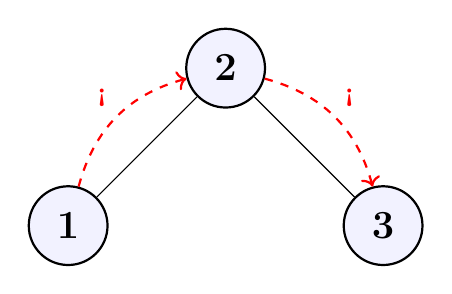
\begin{tikzpicture}[
    treenode/.style = {circle, draw=black, thick, minimum size=10mm, font=\Large\bfseries, fill=blue!5},
    level 1/.style = {sibling distance=4cm, level distance=2cm}
]

\node [treenode] (root) {2}
    child {node [treenode] (left) {1}}
    child {node [treenode] (right) {3}};

\draw[->, dashed, red, thick] (left) to[bend left=30] 
    node[midway, above left, draw=none, font=\small\bfseries, text=red] {<} (root);

\draw[->, dashed, red, thick] (root) to[bend left=30] 
    node[midway, above right, draw=none, font=\small\bfseries, text=red] {<} (right);

\end{tikzpicture}
\end{center}

An insertion always fits into the correct position without violating the inorder order, and a deletion always replaces an internal node with the minimum node in its right subtree to a leaf deletion.

A \textbf{Balanced Search Tree} is a search tree whose subtree heights are balanced to some extent (could be \emph{strictly} or \emph{unstrictly}).

\vspace{2ex}

\textbf{a) AVL Tree}

An \textbf{AVL Tree} is a balanced BST where the height difference between the left and right subtrees of any node is \emph{strictly} at most $1$.

We introduce four types of \emph{rotation}. Denote the current node by $\text X$, the parent by $\text Y$, and the grandparent by $\text Z$.

\begin{figure}[htbp]
    \centering
    \resizebox{\textwidth}{!}{
    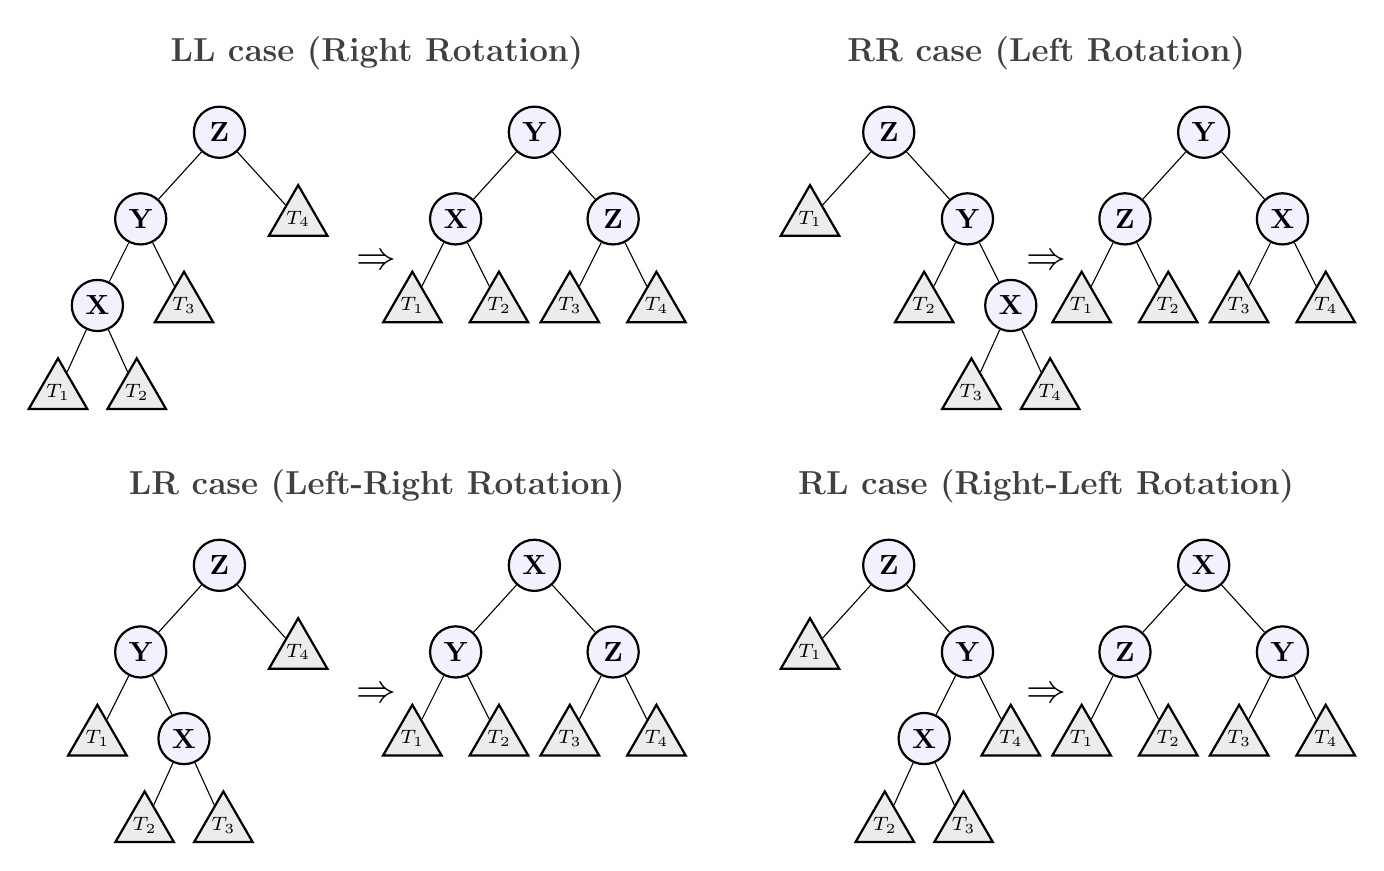
\begin{tikzpicture}[
        treenode/.style = {circle, draw=black, thick, minimum size=6.5mm, font=\normalsize\bfseries, fill=blue!5, inner sep=0pt},
        subtree/.style = {regular polygon, regular polygon sides=3, draw=black, thick, minimum size=8mm, fill=gray!15, inner sep=0pt, font=\scriptsize},
        level 1/.style = {sibling distance=20mm, level distance=11mm},
        level 2/.style = {sibling distance=11mm, level distance=11mm},
        level 3/.style = {sibling distance=10mm, level distance=11mm}
    ]

    \begin{scope}[shift={(0,0)}]
        \node[font=\large\bfseries, text=darkgray] at (2, 1) {LL case (Right Rotation)};
        
        \node [treenode] at (0,0) {Z}
            child {node [treenode] {Y}
                child {node [treenode] {X}
                    child {node [subtree] {$T_1$}}
                    child {node [subtree] {$T_2$}}
                }
                child {node [subtree] {$T_3$}}
            }
            child {node [subtree] {$T_4$}};
            
        \node at (2, -1.65) {\Large $\Rightarrow$};
        
        \node [treenode] at (4,0) {Y}
            child {node [treenode] {X}
                child {node [subtree] {$T_1$}}
                child {node [subtree] {$T_2$}}
            }
            child {node [treenode] {Z}
                child {node [subtree] {$T_3$}}
                child {node [subtree] {$T_4$}}
            };
    \end{scope}

    \begin{scope}[shift={(8.5,0)}] 
        \node[font=\large\bfseries, text=darkgray] at (2, 1) {RR case (Left Rotation)};
        
        \node [treenode] at (0,0) {Z}
            child {node [subtree] {$T_1$}}
            child {node [treenode] {Y}
                child {node [subtree] {$T_2$}}
                child {node [treenode] {X}
                    child {node [subtree] {$T_3$}}
                    child {node [subtree] {$T_4$}}
                }
            };
            
        \node at (2, -1.65) {\Large $\Rightarrow$};
        
        \node [treenode] at (4,0) {Y}
            child {node [treenode] {Z}
                child {node [subtree] {$T_1$}}
                child {node [subtree] {$T_2$}}
            }
            child {node [treenode] {X}
                child {node [subtree] {$T_3$}}
                child {node [subtree] {$T_4$}}
            };
    \end{scope}

    \begin{scope}[shift={(0,-5.5)}] 
        \node[font=\large\bfseries, text=darkgray] at (2, 1) {LR case (Left-Right Rotation)};
        
        \node [treenode] at (0,0) {Z}
            child {node [treenode] {Y}
                child {node [subtree] {$T_1$}}
                child {node [treenode] {X}
                    child {node [subtree] {$T_2$}}
                    child {node [subtree] {$T_3$}}
                }
            }
            child {node [subtree] {$T_4$}};
            
        \node at (2, -1.65) {\Large $\Rightarrow$};
        
        \node [treenode] at (4,0) {X}
            child {node [treenode] {Y}
                child {node [subtree] {$T_1$}}
                child {node [subtree] {$T_2$}}
            }
            child {node [treenode] {Z}
                child {node [subtree] {$T_3$}}
                child {node [subtree] {$T_4$}}
            };
    \end{scope}

    \begin{scope}[shift={(8.5,-5.5)}]
        \node[font=\large\bfseries, text=darkgray] at (2, 1) {RL case (Right-Left Rotation)};
        
        \node [treenode] at (0,0) {Z}
            child {node [subtree] {$T_1$}}
            child {node [treenode] {Y}
                child {node [treenode] {X}
                    child {node [subtree] {$T_2$}}
                    child {node [subtree] {$T_3$}}
                }
                child {node [subtree] {$T_4$}}
            };
            
        \node at (2, -1.65) {\Large $\Rightarrow$};
        
        \node [treenode] at (4,0) {X}
            child {node [treenode] {Z}
                child {node [subtree] {$T_1$}}
                child {node [subtree] {$T_2$}}
            }
            child {node [treenode] {Y}
                child {node [subtree] {$T_3$}}
                child {node [subtree] {$T_4$}}
            };
    \end{scope}

    \end{tikzpicture}
    }
\end{figure}

\textbf{Note:} An insertion takes at most two rotations (can restore the subtree to its original height, as seen in four cases), but a deletion may take $\mathcal O(\log n)$ rotations (e.g. deleting an inner leaf can trigger a rotation, after which the opposite subtree of an ancestor can become two levels taller than the current subtree).

\vspace{2ex}

\textbf{b) Red-Black Tree}

Why am I highlighting this? Because it refers to \texttt{std::map} and \texttt{std::set}, which are common in C++ but do not exist in Python. \textbf{Red-Black Trees} outperform AVL trees in many ways.

We define the root and the leaves to be \emph{black}, and every \emph{red} node must have black children. The core is that every path with the same \textbf{black height} (ending at a black node) must have the same number of black nodes.

\textbf{Therefore}, the longest path cannot be more than twice the length of the shortest path. Since any inserted node must be red, rotation only occurs when the inserted node's parent is red.

We introduce \emph{color flip}. Denote the current node by $\text N$, the parent by $\text P$, the uncle by $\text U$, and the grandparent by $\text G$.

\begin{figure}[H]
    \centering
    \resizebox{\textwidth}{!}{
    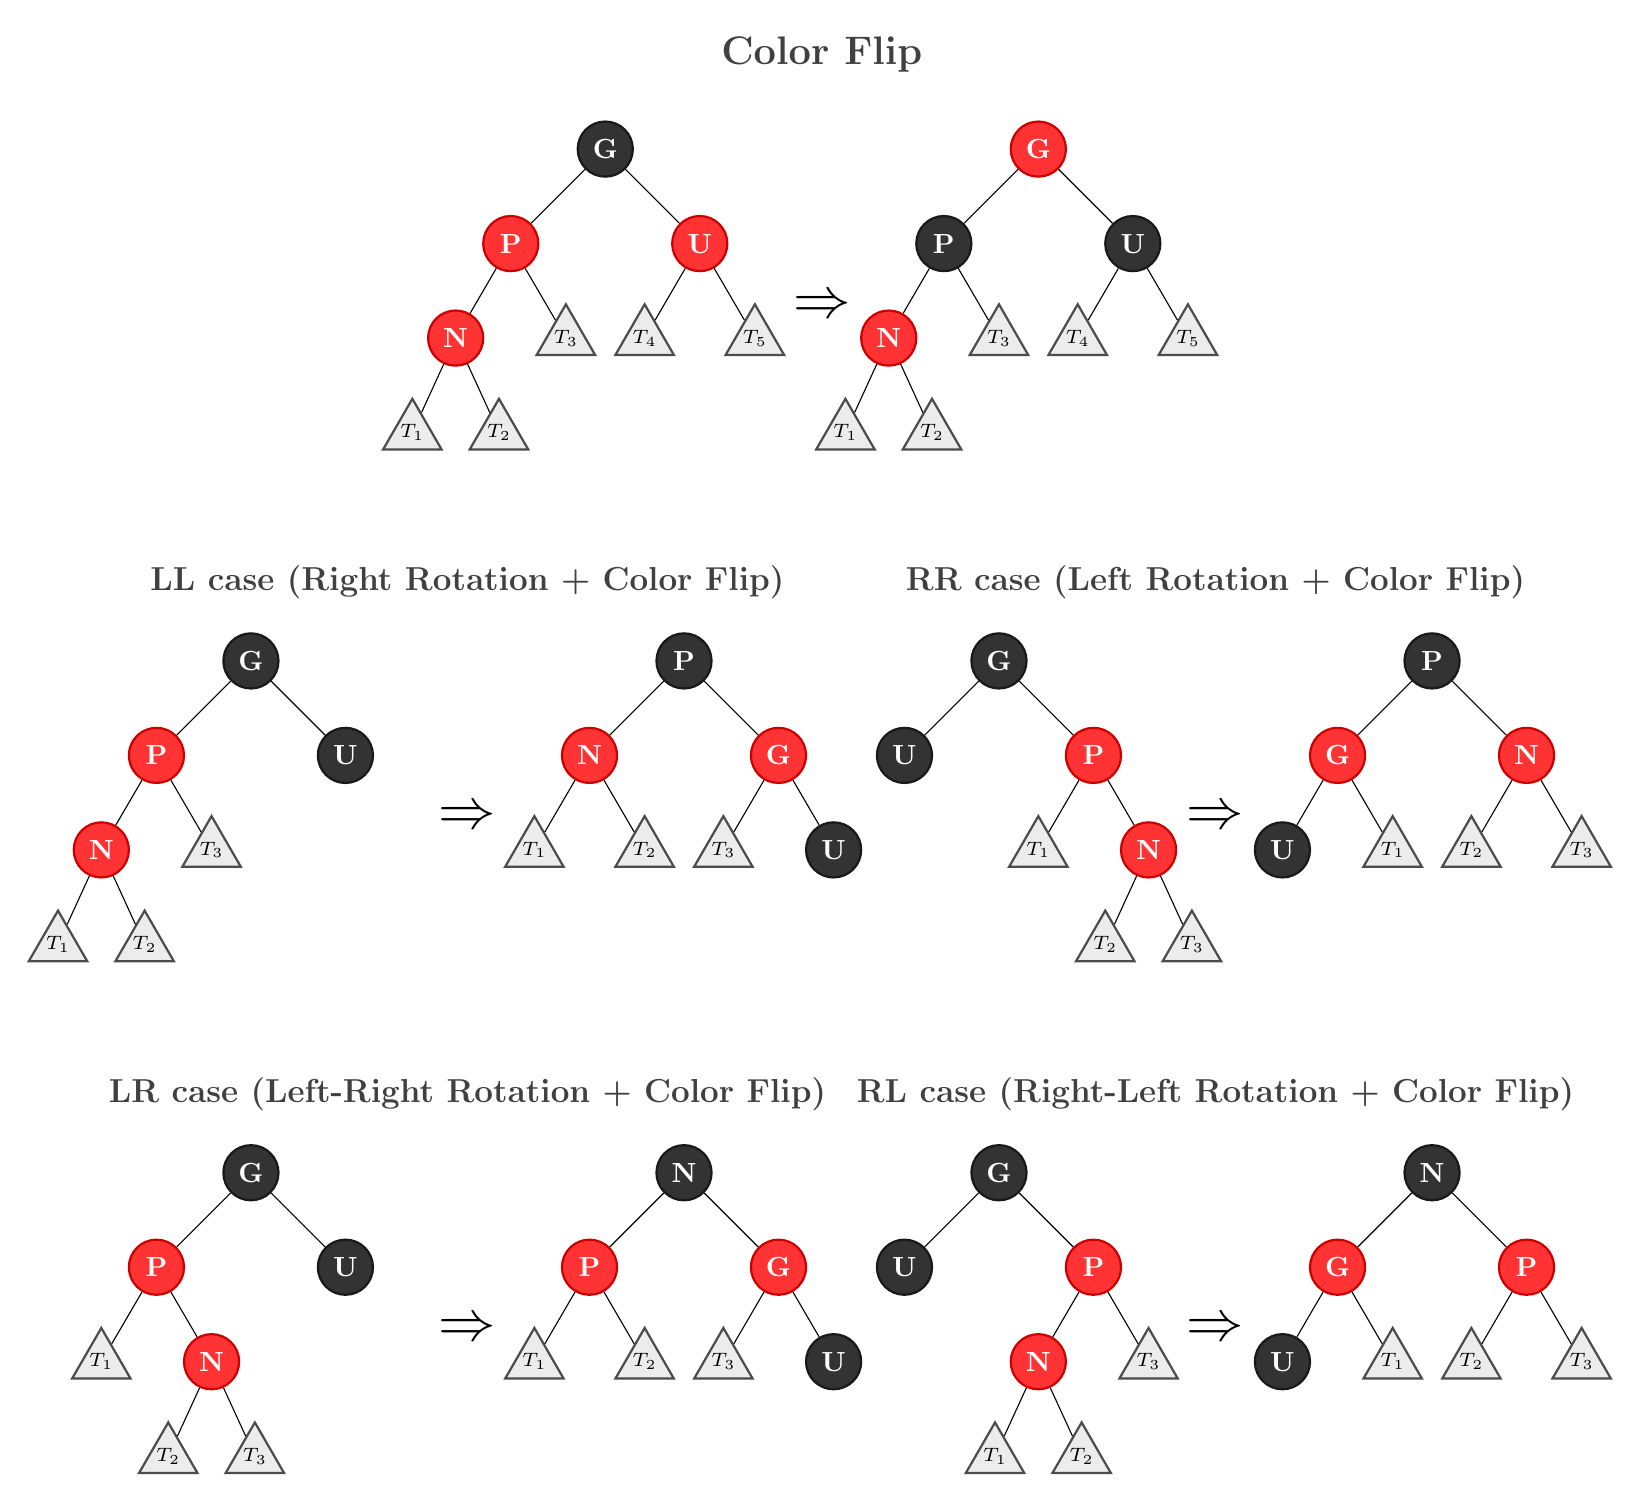
\begin{tikzpicture}[
        bnode/.style = {circle, draw=black!90, thick, minimum size=7mm, font=\normalsize\bfseries, fill=black!80, text=white, inner sep=0pt},
        rnode/.style = {circle, draw=red!80!black, thick, minimum size=7mm, font=\normalsize\bfseries, fill=red!80, text=white, inner sep=0pt},
        subtree/.style = {regular polygon, regular polygon sides=3, draw=black!70, thick, minimum size=8.5mm, fill=gray!15, inner sep=0pt, font=\scriptsize},
        level 1/.style = {sibling distance=24mm, level distance=12mm},
        level 2/.style = {sibling distance=14mm, level distance=12mm},
        level 3/.style = {sibling distance=11mm, level distance=12mm}
    ]

    \begin{scope}[shift={(4.5,0)}]
        \node[font=\Large\bfseries, text=darkgray] at (2.75, 1.2) {Color Flip};
        
        \node [bnode] at (0,0) {G}
            child {node [rnode] {P}
                child {node [rnode] {N}
                    child {node [subtree] {$T_1$}}
                    child {node [subtree] {$T_2$}}
                }
                child {node [subtree] {$T_3$}}
            }
            child {node [rnode] {U}
                child {node [subtree] {$T_4$}}
                child {node [subtree] {$T_5$}}
            };
            
        \node at (2.75, -2) {\huge $\Rightarrow$};
        
        \node [rnode] at (5.5,0) {G}
            child {node [bnode] {P}
                child {node [rnode] {N}
                    child {node [subtree] {$T_1$}}
                    child {node [subtree] {$T_2$}}
                }
                child {node [subtree] {$T_3$}}
            }
            child {node [bnode] {U}
                child {node [subtree] {$T_4$}}
                child {node [subtree] {$T_5$}}
            };
    \end{scope}

    \begin{scope}[shift={(0,-6.5)}]
        \node[font=\large\bfseries, text=darkgray] at (2.75, 1) {LL case (Right Rotation + Color Flip)};
        
        \node [bnode] at (0,0) {G}
            child {node [rnode] {P}
                child {node [rnode] {N}
                    child {node [subtree] {$T_1$}}
                    child {node [subtree] {$T_2$}}
                }
                child {node [subtree] {$T_3$}}
            }
            child {node [bnode] {U}};
            
        \node at (2.75, -2) {\huge $\Rightarrow$};
        
        \node [bnode] at (5.5,0) {P}
            child {node [rnode] {N}
                child {node [subtree] {$T_1$}}
                child {node [subtree] {$T_2$}}
            }
            child {node [rnode] {G}
                child {node [subtree] {$T_3$}}
                child {node [bnode] {U}}
            };
    \end{scope}

    \begin{scope}[shift={(9.5,-6.5)}]
        \node[font=\large\bfseries, text=darkgray] at (2.75, 1) {RR case (Left Rotation + Color Flip)};
        
        \node [bnode] at (0,0) {G}
            child {node [bnode] {U}}
            child {node [rnode] {P}
                child {node [subtree] {$T_1$}}
                child {node [rnode] {N}
                    child {node [subtree] {$T_2$}}
                    child {node [subtree] {$T_3$}}
                }
            };
            
        \node at (2.75, -2) {\huge $\Rightarrow$};
        
        \node [bnode] at (5.5,0) {P}
            child {node [rnode] {G}
                child {node [bnode] {U}}
                child {node [subtree] {$T_1$}}
            }
            child {node [rnode] {N}
                child {node [subtree] {$T_2$}}
                child {node [subtree] {$T_3$}}
            };
    \end{scope}

    \begin{scope}[shift={(0,-13)}]
        \node[font=\large\bfseries, text=darkgray] at (2.75, 1) {LR case (Left-Right Rotation + Color Flip)};
        
        \node [bnode] at (0,0) {G}
            child {node [rnode] {P}
                child {node [subtree] {$T_1$}}
                child {node [rnode] {N}
                    child {node [subtree] {$T_2$}}
                    child {node [subtree] {$T_3$}}
                }
            }
            child {node [bnode] {U}};
            
        \node at (2.75, -2) {\huge $\Rightarrow$};
        
        \node [bnode] at (5.5,0) {N}
            child {node [rnode] {P}
                child {node [subtree] {$T_1$}}
                child {node [subtree] {$T_2$}}
            }
            child {node [rnode] {G}
                child {node [subtree] {$T_3$}}
                child {node [bnode] {U}}
            };
    \end{scope}

    \begin{scope}[shift={(9.5,-13)}]
        \node[font=\large\bfseries, text=darkgray] at (2.75, 1) {RL case (Right-Left Rotation + Color Flip)};
        
        \node [bnode] at (0,0) {G}
            child {node [bnode] {U}}
            child {node [rnode] {P}
                child {node [rnode] {N}
                    child {node [subtree] {$T_1$}}
                    child {node [subtree] {$T_2$}}
                }
                child {node [subtree] {$T_3$}}
            };
            
        \node at (2.75, -2) {\huge $\Rightarrow$};
        
        \node [bnode] at (5.5,0) {N}
            child {node [rnode] {G}
                child {node [bnode] {U}}
                child {node [subtree] {$T_1$}}
            }
            child {node [rnode] {P}
                child {node [subtree] {$T_2$}}
                child {node [subtree] {$T_3$}}
            };
    \end{scope}

    \end{tikzpicture}
    }
\end{figure}

\textbf{Note:} An insertion takes at most two rotations (can restore the subtree to its original black height, as seen in five cases), and a deletion takes at most three rotations (e.g. deleting a black node whose sibling is red can first require a left rotation, followed by an RL case that requires two rotations).

\textbf{c) B-Tree}

A \textbf{B-Tree} is a strictly balanced \emph{Multiway Search Tree (MST)}. The \emph{order} $m$ denotes the maximum number of children per node, therefore each node can store at most $m−1$ keys (shown below for $m=3$). Only when the root splits does the height increase by one, otherwise it remains unchanged.

\vspace{-1ex}

\begin{center}
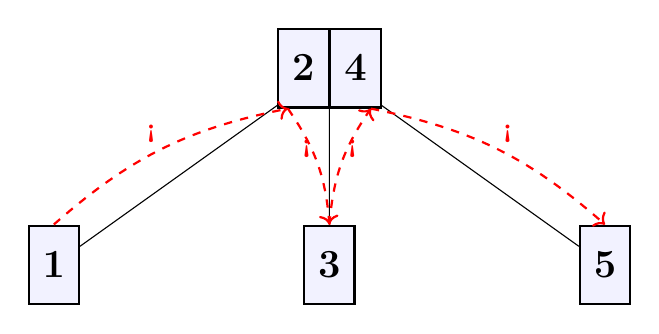
\begin{tikzpicture}[
    btree node/.style = {
        rectangle split, 
        rectangle split horizontal,
        rectangle split parts=#1,
        draw=black, 
        thick, 
        minimum height=10mm, 
        font=\Large\bfseries, 
        fill=blue!5,
        inner sep=5pt
    },
    level 1/.style = {sibling distance=3.5cm, level distance=2.5cm}
]

\node [btree node=2] (root) {2 \nodepart{two} 4}
    child {node [btree node=1] (child1) {1}}
    child {node [btree node=1] (child2) {3}}
    child {node [btree node=1] (child3) {5}};

\draw[->, dashed, red, thick] (child1.north) to[bend left=15] 
    node[midway, above left=-2pt, draw=none, font=\small\bfseries, text=red] {<} ([xshift=-15pt]root.south);

\draw[->, dashed, red, thick] ([xshift=-15pt]root.south) to[bend right=-15] 
    node[midway, above left=-2pt, draw=none, font=\small\bfseries, text=red] {<} (child2.north);

\draw[->, dashed, red, thick] (child2.north) to[bend left=15] 
    node[midway, above right=-2pt, draw=none, font=\small\bfseries, text=red] {<} ([xshift=15pt]root.south);

\draw[->, dashed, red, thick] ([xshift=15pt]root.south) to[bend right=-15] 
    node[midway, above right=-2pt, draw=none, font=\small\bfseries, text=red] {<} (child3.north);

\end{tikzpicture}
\end{center}

\textbf{d) B+ Tree}

A \textbf{B+ Tree} is also a strictly balanced MST. Only the leaves store data --- the internal nodes are purely indices (not real data). The leaves at the bottom are stored in a \emph{doubly linked list}.

\begin{center}
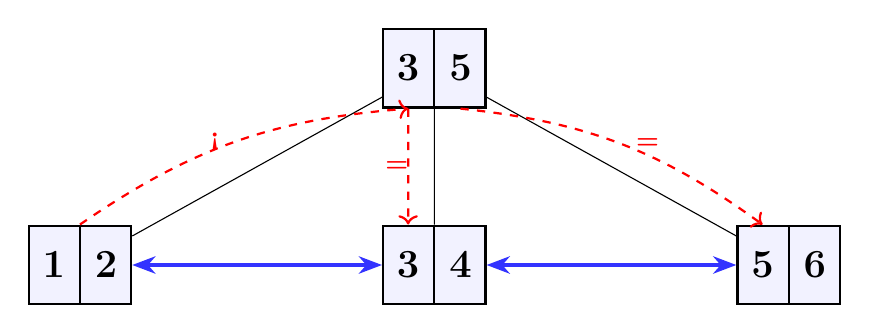
\begin{tikzpicture}[
    btree node/.style = {
        rectangle split, 
        rectangle split horizontal,
        rectangle split parts=#1,
        draw=black, 
        thick, 
        minimum height=10mm, 
        font=\Large\bfseries, 
        fill=blue!5,
        inner sep=5pt
    },
    level 1/.style = {sibling distance=4.5cm, level distance=2.5cm}
]

\node [btree node=2] (root) {3 \nodepart{two} 5}
    child {node [btree node=2] (leaf1) {1 \nodepart{two} 2}}
    child {node [btree node=2] (leaf2) {3 \nodepart{two} 4}}
    child {node [btree node=2] (leaf3) {5 \nodepart{two} 6}};

\draw[<->, >=Stealth, very thick, blue!80] (leaf1.east) -- (leaf2.west)
    node[midway, above, font=\scriptsize\bfseries, text=blue!80] {};
    
\draw[<->, >=Stealth, very thick, blue!80] (leaf2.east) -- (leaf3.west)
    node[midway, above, font=\scriptsize\bfseries, text=blue!80] {};

\draw[->, dashed, red, thick] (leaf1.north) to[bend left=15] 
    node[midway, left=2pt, draw=none, font=\small\bfseries, text=red] {<} (root.one south);

\draw[->, dashed, red, thick] (root.one south) to[bend right=0] 
    node[midway, right=-12pt, draw=none, font=\small\bfseries, text=red] {=} (leaf2.one north);

\draw[->, dashed, red, thick] (root.two south) to[bend left=15] 
    node[midway, right=2pt, draw=none, font=\small\bfseries, text=red] {=} (leaf3.one north);

\end{tikzpicture}
\end{center}


\textbf{e) B* Tree}

A \textbf{B* Tree} is a B+ Tree. Not only are the leaves at the bottom stored in a doubly linked list, but so are the nodes at every level. If a node is full, it \emph{gives} some of its keys to a sibling before splitting.

\begin{center}
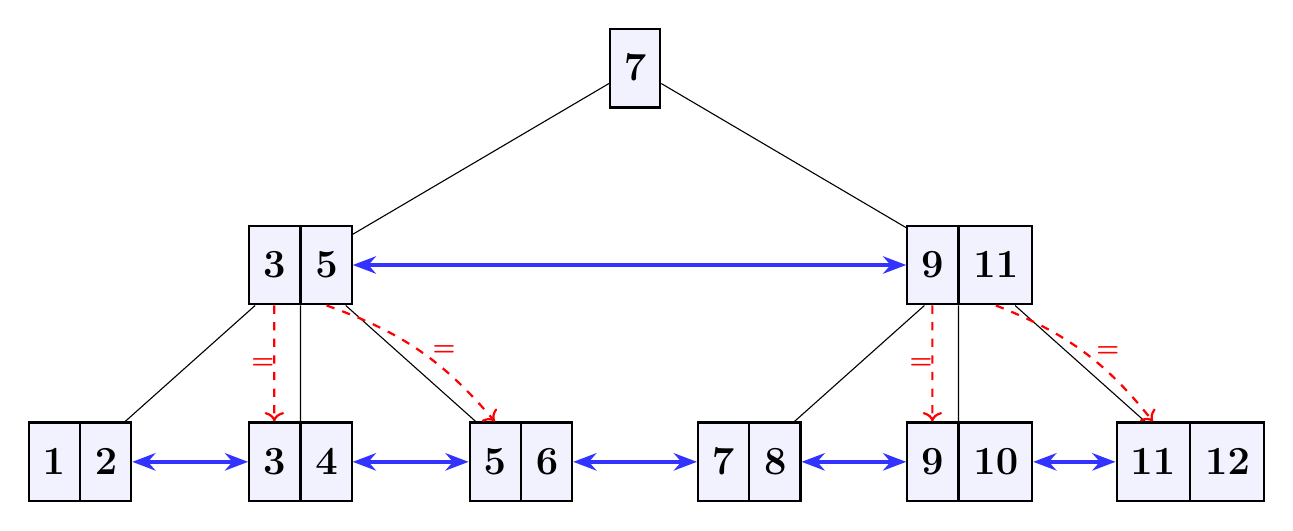
\begin{tikzpicture}[
    btree node/.style = {
        rectangle split, 
        rectangle split horizontal,
        rectangle split parts=#1,
        draw=black, 
        thick, 
        minimum height=10mm, 
        font=\Large\bfseries, 
        fill=blue!5,
        inner sep=5pt
    },
    level 1/.style = {sibling distance=8.5cm, level distance=2.5cm},
    level 2/.style = {sibling distance=2.8cm, level distance=2.5cm},
    sibling ptr/.style = {<->, >=Stealth, very thick, blue!80}
]

\node [btree node=1] (root) {7}
    child {node [btree node=2] (int1) {3 \nodepart{two} 5}
        child {node [btree node=2] (leaf1) {1 \nodepart{two} 2}}
        child {node [btree node=2] (leaf2) {3 \nodepart{two} 4}}
        child {node [btree node=2] (leaf3) {5 \nodepart{two} 6}}
    }
    child {node [btree node=2] (int2) {9 \nodepart{two} 11}
        child {node [btree node=2] (leaf4) {7 \nodepart{two} 8}}
        child[edge from parent path={(\tikzparentnode.one split south) -- (\tikzchildnode.one split north)}] {node [btree node=2] (leaf5) {9 \nodepart{two} 10}}
        child {node [btree node=2] (leaf6) {11 \nodepart{two} 12}}
    };

\draw[sibling ptr] (int1.east) -- (int2.west) 
    node[midway, above, font=\small\bfseries, text=blue!80] {};

\draw[sibling ptr] (leaf1.east) -- (leaf2.west);
\draw[sibling ptr] (leaf2.east) -- (leaf3.west);
\draw[sibling ptr] (leaf3.east) -- (leaf4.west); 
\draw[sibling ptr] (leaf4.east) -- (leaf5.west);
\draw[sibling ptr] (leaf5.east) -- (leaf6.west);

\draw[->, dashed, red, thick] (int1.one south) to[bend right=0] 
    node[midway, right=-12pt, draw=none, font=\small\bfseries, text=red] {=} (leaf2.one north);
\draw[->, dashed, red, thick] (int1.two south) to[bend left=15] 
    node[midway, right=1pt, draw=none, font=\small\bfseries, text=red] {=} (leaf3.one north);

\draw[->, dashed, red, thick] (int2.one south) to[bend right=0] 
    node[midway, right=-12pt, draw=none, font=\small\bfseries, text=red] {=} (leaf5.one north);
\draw[->, dashed, red, thick] (int2.two south) to[bend left=15] 
    node[midway, right=1pt, draw=none, font=\small\bfseries, text=red] {=} (leaf6.one north);

\end{tikzpicture}
\end{center}

\vspace{4ex}

\subsubsection{Fenwick Tree}

A \textbf{Fenwick Tree} is also called a \emph{Binary Indexed Tree (BIT)}. Before we start with it, we shall first introduce \emph{prefix sums} and \emph{suffix sums}.

\begin{Question}{Subarray Sum Equals K $\bigstar$}
Given an array of integers nums and an integer \texttt{K}, return the total number of subarrays whose sum equals to \texttt{K}. A subarray is a contiguous non-empty sequence of elements within an array.
\end{Question}

A subarray sum is the difference between two prefix sums. From this idea, we only need to store all prefix sums in a hashmap. In this way, we can solve the problem in a single $\mathcal O(n)$ pass.

\begin{lstlisting}[style=python]
class Solution:
    def subarraySum(self, nums: List[int], k: int) -> int:
        m = {}
        ans = 0
        sum = 0
        
        for num in nums:
            if sum in m:
                m[sum] += 1
            else:
                m[sum] = 1
            sum += num
            if sum - k in m:
                ans += m[sum - k]
                
        return ans
\end{lstlisting}

\begin{Question}{Count of Smaller Numbers After Self $\bigstar\bigstar\bigstar$}
Given an integer array \texttt{nums}, return an integer array counts where \texttt{counts[i]} is the number of smaller elements to the right of \texttt{nums[i]}.
\end{Question}

Intuitively, we can start from the right side, adding one to every key in the hashtable that is greater than the current number --- however this is \textbf{IMPOSSIBLE} because the range of numbers is too large, and each update would take $\mathcal{O}(n)$ time!

In fact, the first problem is easy to solve using \emph{discretization}. How can we reduce the second problem to $\mathcal{O}(\log n)$? Hint: we need to add one to a range at each step.

Now it is time to introduce Fenwick Trees.

\begin{center}
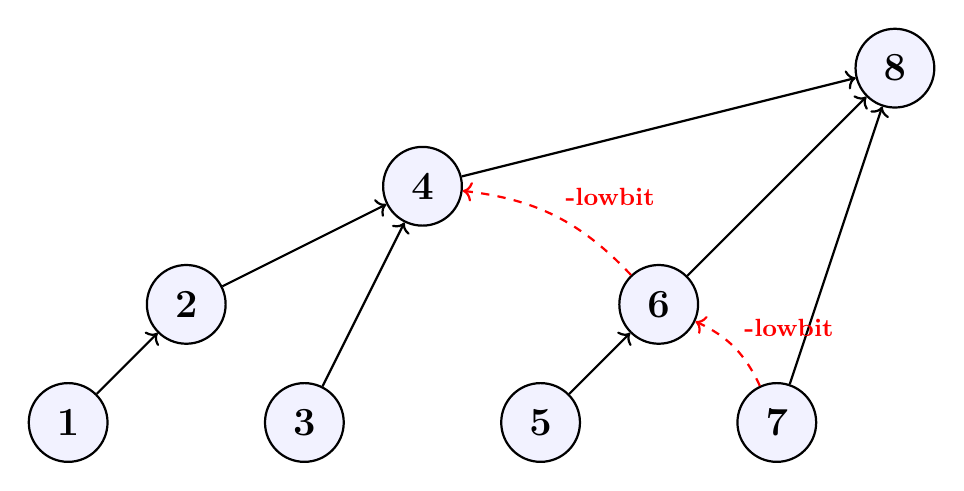
\begin{tikzpicture}[
    treenode/.style = {circle, draw=black, thick, minimum size=10mm, font=\Large\bfseries, fill=blue!5},
    xscale=1.5, yscale=1.5
]

\node [treenode] (n1) at (1, 0) {1};
\node [treenode] (n3) at (3, 0) {3};
\node [treenode] (n5) at (5, 0) {5};
\node [treenode] (n7) at (7, 0) {7};

\node [treenode] (n2) at (2, 1) {2};
\node [treenode] (n6) at (6, 1) {6};

\node [treenode] (n4) at (4, 2) {4};

\node [treenode] (n8) at (8, 3) {8};

\draw[->, thick] (n1) -- (n2);
\draw[->, thick] (n2) -- (n4);
\draw[->, thick] (n3) -- (n4);
\draw[->, thick] (n4) -- (n8);
\draw[->, thick] (n5) -- (n6);
\draw[->, thick] (n6) -- (n8);
\draw[->, thick] (n7) -- (n8);

\draw[->, dashed, red, thick] (n7) to[bend right=20] 
    node[midway, above right, draw=none, font=\small\bfseries, text=red] {-lowbit} (n6);

\draw[->, dashed, red, thick] (n6) to[bend right=20] 
    node[midway, above right, draw=none, font=\small\bfseries, text=red] {-lowbit} (n4);

\end{tikzpicture}
\end{center}

This is a classical prefix Fenwick Tree using 1-based indexing. So please don't forget to add $1$, since arrays start counting from $0$.

There is a \emph{lowbit} trick called \texttt{lowbit(i)=i\&(-i)}, which extracts the least significant set bit. During an element update we recursively apply \texttt{i+=lowbit(i)}, whereas during a range query we recursively apply \texttt{i-=lowbit(i)}.

\begin{lstlisting}[style=python]
class Solution:
    def lowbit(self, x: int) -> int:
        return x & (-x)

    def add(self, index: int, delta: int) -> None:
        i = index + 1
        while i <= self.N:
            self.fenwick[i] += delta
            i += self.lowbit(i)

    def query(self, index: int) -> int:
        val = 0
        i = index + 1
        
        while i > 0:
            val += self.fenwick[i]
            i -= self.lowbit(i)
            
        return val

    def countSmaller(self, nums: list[int]) -> list[int]:
        n = len(nums)
        ans = [0] * n
        discrete_nums = sorted(list(set(nums)))
        self.N = len(discrete_nums)
        self.fenwick = [0] * (self.N + 1)
        
        for i in range(n - 1, -1, -1):
            rank = bisect.bisect_left(discrete_nums, nums[i]) + 1
            ans[i] = self.query(rank - 1)
            self.add(rank, 1)
            
        return ans
\end{lstlisting}

The situation above involves adding new elements to a Fenwick Tree while querying a range sum at the same time. But what if we only need to convert a normal array into a Fenwick Tree? Instead of updating each element in $\mathcal{O}(n\log n)$ time, we can build it in $\mathcal{O}(n)$ time.

\begin{lstlisting}[style=python]
for i in range(1, n + 1):
    par = i + lowbit(i)
    if par <= n:
        fenwick[par] += fenwick[i]
\end{lstlisting}

This is the so-called \textbf{Contribution Technique}.

In fact, Fenwick Trees can also be used for range additions. See the following problem.

\begin{Question}{Interval Fenwick $\bigstar\bigstar\bigstar\bigstar\bigstar$}
Design a data structure that efficiently supports range updates and prefix sum queries.

Implement the \texttt{IntervalFenwick} class:

\begin{itemize}
    \item \texttt{IntervalFenwick(int n)} initializes the data structure with an array of size \texttt{n} containing all \texttt{0}s.
    \item \texttt{void updateRange(int left, int right, int value)} adds value to all elements in the inclusive range \texttt{[left,right]}.
    \item \texttt{int queryRange(int index)} returns the sum of all elements in the inclusive prefix range \texttt{[1,index]}.
\end{itemize}
\end{Question}

How can we \emph{transform} range updates into point updates?

Use \emph{Abel's Transformation} as a tool! Let's say we use $A[i]$ as the original array. We take its derivative (technically, the difference), the sum query becomes:

$$
\sum_{i=1}^x A[i]\cdot 1=x\cdot A[x]-\sum_{i=1}^{x-1}i\Delta A[i]=x\left(\sum_{i=1}^{x-1}\Delta A[i]+A[1]\right)-\sum_{i=1}^{x-1}i\Delta A[i].
$$

Simplify this using $\Delta A[i]=D[i+1]$:

$$
x\left(\sum_{i=1}^{x-1}\Delta A[i]+A[1]\right)-\sum_{i=1}^{x-1}i\Delta A[i]=(x+1)\sum_{i=1}^x D[i]-\sum_{i=1}^x iD[i].
$$

We only need to update the two range boundaries rather than the whole range. Moreover, for a range query, we calculate the prefix sum by querying $D[i]$ and $iD[i]$ which represent two Fenwick Trees.

\begin{lstlisting}[style=python]
class IntervalFenwick:
    def __init__(self, n: int):
        self.n = n
        self.d1 = [0] * (n + 2)
        self.d2 = [0] * (n + 2)

    def lowbit(self, x: int) -> int:
        return x & (-x)

    def add(self, tree: list[int], index: int, delta: int) -> None:
        while index <= self.n + 1:
            tree[index] += delta
            index += self.lowbit(index)

    def query(self, tree: list[int], index: int) -> int:
        res = 0
        
        while index > 0:
            res += tree[index]
            index -= self.lowbit(index)
            
        return res

    def updateRange(self, left: int, right: int, value: int) -> None:
        self.add(self.d1, left, value)
        self.add(self.d1, right + 1, -value)
        self.add(self.d2, left, left * value)
        self.add(self.d2, right + 1, (right + 1) * (-value))

    def queryRange(self, index: int) -> int:
        sum_d1 = self.query(self.d1, index)
        sum_d2 = self.query(self.d2, index)
        return (index + 1) * sum_d1 - sum_d2
\end{lstlisting}


\subsubsection{Segment Tree}

\textbf{Segment Trees} are slightly slower than Fenwick Trees in terms of constant factors but they are much more general, especially for range updates (see propagation below). A segment tree is a balanced binary tree.

Why do we call them segment trees? Because each node represents an interval of indices, or, a segment of the index range.

\begin{center}
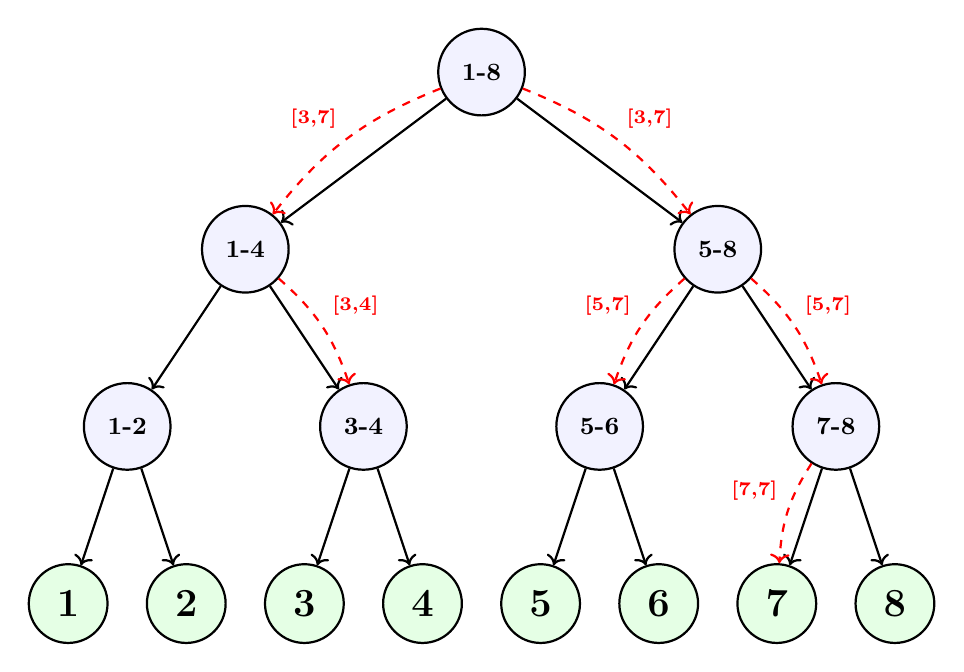
\begin{tikzpicture}[
    treenode/.style = {circle, draw=black, thick, minimum size=11mm, font=\small\bfseries, fill=blue!5},
    leafnode/.style = {circle, draw=black, thick, minimum size=10mm, font=\Large\bfseries, fill=green!10},
    xscale=1.5, yscale=1.5
]

\node [leafnode] (n1) at (1, 0) {1};
\node [leafnode] (n2) at (2, 0) {2};
\node [leafnode] (n3) at (3, 0) {3};
\node [leafnode] (n4) at (4, 0) {4};
\node [leafnode] (n5) at (5, 0) {5};
\node [leafnode] (n6) at (6, 0) {6};
\node [leafnode] (n7) at (7, 0) {7};
\node [leafnode] (n8) at (8, 0) {8};

\node [treenode] (n12) at (1.5, 1.5) {1-2};
\node [treenode] (n34) at (3.5, 1.5) {3-4};
\node [treenode] (n56) at (5.5, 1.5) {5-6};
\node [treenode] (n78) at (7.5, 1.5) {7-8};

\node [treenode] (n14) at (2.5, 3) {1-4};
\node [treenode] (n58) at (6.5, 3) {5-8};

\node [treenode] (n18) at (4.5, 4.5) {1-8};

\draw[->, thick] (n18) -- (n14);
\draw[->, thick] (n18) -- (n58);

\draw[->, thick] (n14) -- (n12);
\draw[->, thick] (n14) -- (n34);
\draw[->, thick] (n58) -- (n56);
\draw[->, thick] (n58) -- (n78);

\draw[->, thick] (n12) -- (n1);
\draw[->, thick] (n12) -- (n2);
\draw[->, thick] (n34) -- (n3);
\draw[->, thick] (n34) -- (n4);
\draw[->, thick] (n56) -- (n5);
\draw[->, thick] (n56) -- (n6);
\draw[->, thick] (n78) -- (n7);
\draw[->, thick] (n78) -- (n8);

\draw[->, dashed, red, thick] (n18) to[bend right=15] 
    node[midway, above left, text=red, font=\scriptsize\bfseries] {[3,7]} (n14);
\draw[->, dashed, red, thick] (n18) to[bend left=15] 
    node[midway, above right, text=red, font=\scriptsize\bfseries] {[3,7]} (n58);

\draw[->, dashed, red, thick] (n14) to[bend left=15] 
    node[midway, above right, text=red, font=\scriptsize\bfseries] {[3,4]} (n34);

\draw[->, dashed, red, thick] (n58) to[bend right=15] 
    node[midway, above left, text=red, font=\scriptsize\bfseries] {[5,7]} (n56);
\draw[->, dashed, red, thick] (n58) to[bend left=15] 
    node[midway, above right, text=red, font=\scriptsize\bfseries] {[5,7]} (n78);

\draw[->, dashed, red, thick] (n78) to[bend right=15] 
    node[midway, above left, text=red, font=\scriptsize\bfseries] {[7,7]} (n7);

\end{tikzpicture}
\end{center}

If a node is completely included in the range to be updated, it immediately stops propagating and adds a \emph{lazy tag} to itself. Only when another operation (either an update or a query) reaches this node is the lazy tag pushed down to its children.

This is called \textbf{Lazy Algorithm} (last but not least, lazy algorithms are applied to, but not limited to Segment Trees, DSUs, Dijkstra's Algorithm, etc.).

\begin{lstlisting}[style=python]
class SegmentTree:
    def __init__(self, n: int):
        self.segment = [0] * (4 * n)
        self.mark = [0] * (4 * n)

    def pushdown(self, p: int, cl: int, cr: int) -> None:
        mid = (cl + cr) // 2
        left_child = 2 * p
        right_child = 2 * p + 1
        self.mark[left_child] += self.mark[p]
        self.segment[left_child] += self.mark[p] * (mid - cl + 1)
        self.mark[right_child] += self.mark[p]
        self.segment[right_child] += self.mark[p] * (cr - mid)
        self.mark[p] = 0

    def query(self, l: int, r: int, p: int, cl: int, cr: int) -> int:
        if cl > r or cr < l:
            return 0
        if cl >= l and cr <= r:
            return self.segment[p]
        self.pushdown(p, cl, cr)
        mid = (cl + cr) // 2
        return self.query(l, r, 2 * p, cl, mid) + self.query(l, r, 2 * p + 1, mid + 1, cr)

    def update(self, l: int, r: int, val: int, p: int, cl: int, cr: int) -> None:
        if cr < l or cl > r:
            return
        if cl >= l and cr <= r:
            self.segment[p] += val * (cr - cl + 1)
            self.mark[p] += val
            return
        mid = (cl + cr) // 2
        self.pushdown(p, cl, cr)
        self.update(l, r, val, 2 * p, cl, mid)
        self.update(l, r, val, 2 * p + 1, mid + 1, cr)
        self.segment[p] = self.segment[2 * p] + self.segment[2 * p + 1]
\end{lstlisting}

We use an $\mathcal O(2n)$ way to build a segment tree, and this is a very typical example of \emph{Divide and Conquer}:

\begin{lstlisting}[style=python]
def build(self, l: int, r: int, p: int) -> None:
    if l == r:
        self.segment[p] = self.nums[l - 1]
        return
    mid = (l + r) // 2
    self.build(l, mid, 2 * p)
    self.build(mid + 1, r, 2 * p + 1)
    self.segment[p] = self.segment[2 * p] + self.segment[2 * p + 1]
\end{lstlisting}

\textbf{Note:} Hmm, don't you think we can skip the pushdown for the update process if the update operation is \emph{commutative}? We can definitely implement this with a better constant factor by a \emph{Permanent Tags} trick!

If we lean more into an abstract algebra view, let's denote the content in the nodes as maintaining an operation $\oplus$, forming a \emph{monoid} with \emph{associativity} $(G, \oplus)$, and the lazy tag as representing a function $f$, which also forms a monoid with associativity $(F, \circ)$. The requirement for a segment tree to hold is equivalent to:$$f(a\oplus b)=f(a)\oplus f(b)$$which is an \emph{endomorphism}. If the lazy tag $(F,\circ)$ is commutative, it is an \emph{Abelian Monoid} that can apply the permanent tags trick.


\subsection{Graph}

\subsubsection{Disjoint Set Union}

Since adjacency lists and adjacency matrices being too straightforward to write much about (and they'll occur in many questions later), I'm going to start with \emph{Set and Union} idea in graph-like data structures first!

It is widely related to, but not limited to minimum spanning tree algorithms, connectivity judgments, etc. We implement the idea using \textbf{Disjoint Set Union (DSU)}.

DSU has two operations: \emph{Union} and \emph{Find}. Every set has a root parent, and commonly we use \emph{path compression} to make the leaves point to the root, keeping the paths as short as possible. \textbf{BUT}, a union operation could trigger a situation where one set's root points to another set's root, yet the leaves of the former have not yet updated to point to this new root. Therefore, even when compression is applied to the class, the tree can still have a depth greater than 2, reflecting the concept of a \emph{lazy algorithm}.

\newpage

\begin{lstlisting}[style=python]
class DSU:
    def __init__(self, n: int):
        self.n = n
        self.par = list(range(n))
        self.rank = [0] * n

    def find(self, x: int) -> int:
        if self.par[x] != x:
            self.par[x] = self.find(self.par[x])
        return self.par[x]

    def merge(self, x: int, y: int) -> bool:
        rx = self.find(x)
        ry = self.find(y)
        if rx == ry:
            return False
        if self.rank[rx] < self.rank[ry]:
            self.par[rx] = ry
        elif self.rank[ry] < self.rank[rx]:
            self.par[ry] = rx
        else:
            self.par[rx] = ry
            self.rank[ry] += 1
        return True
\end{lstlisting}

\begin{Question}{Most Stones Removed with Same Row or Column $\bigstar\bigstar$}
On a 2D plane, we place $\texttt n$ stones at some integer coordinate points. Each coordinate point may have at most one stone.

A stone can be removed if it shares either the same row or the same column as another stone that has not been removed.

Given an array $\texttt{stones}$ of length $\texttt n$ where $\texttt{stones[i]=[x}_\texttt{i}\texttt{,y}_\texttt{i}\texttt{]}$ represents the location of the $\texttt i^{\texttt{th}}$ stone, return the largest possible number of stones that can be removed.
\end{Question}

Translate the problem and we'll see that any stones sharing the same row or column (i.e. a cross pattern) can be reduced to a single stone.

We can store each row in a rowmap and each column in a columnmap, and if we find a new stone whose row or column is already recorded, we then merge it with the corresponding set and increment our answer by one.

\begin{lstlisting}[style=python]
class Solution:
    def removeStones(self, stones: list[list[int]]) -> int:
        n = len(stones)
        rowmap = {}
        colmap = {}
        dsu = DSU(n)
        ans = 0
        
        for idx, (x, y) in enumerate(stones):
            if x not in rowmap:
                rowmap[x] = idx
            else:
                if dsu.merge(idx, rowmap[x]):
                    ans += 1
            if y not in colmap:
                colmap[y] = idx
            else:
                if dsu.merge(idx, colmap[y]):
                    ans += 1
                    
        return ans
\end{lstlisting}

\begin{Question}{Jump DSU $\bigstar\bigstar\bigstar\bigstar$}
Given a binary string \texttt{s}, and an integer \texttt{k}. In one operation, you must choose exactly \texttt{k} different indices and flip each \texttt{'0'} to \texttt{'1'} and each \texttt{'1'} to \texttt{'0'}.

Return the minimum number of operations required to make all characters in the string equal to \texttt{'1'}. If it is not possible, return \texttt{-1}.
\end{Question}

We can't do this with a simple BFS (would require all permutations).

However, the order is not important in this problem --- what about a pruned BFS that only cares about how many \texttt{'0'}s are left? This would be $\mathcal O(n^2)$ overall, with an $\mathcal O(n)$ search space.
Please note that even with a visited boolean check, we still consider the overall complexity as $\mathcal O(V+E) = \mathcal O(V+\mathcal O(V)) = \mathcal O(V^2)$.

Can we, let's suppose, compress the search space? We don't want to evaluate $\mathcal O(n)$ possibilities every single time. Hmm, why not --- what if we link every node directly to its successor (or the next valid successor, whenever appropriate), instead of checking that if-statement every time? It acts like arrows on the same level of BFS spanning tree (e.g. there was $1\rightarrow[2,5]$ before, so for $2\rightarrow[3,6]$ jump $2\rightarrow3\rightarrow6$ without $4,5$).

Note that if we do this, we \textbf{CAN'T} use union by rank --- we are defining the root as the next valid successor node! This is the so-called \textbf{Jump DSU} trick, suitable for BFS in an ordered search space.

\begin{lstlisting}[style=python]
class DSU:
    def __init__(self, n: int):
        self.parent = list(range(n + 3))

    def find(self, i: int) -> int:
        if self.parent[i] != i:
            self.parent[i] = self.find(self.parent[i])
        return self.parent[i]

class Solution:
    def minOperations(self, s: str, k: int) -> int:
        n = len(s)
        init_z = s.count('0')
        if init_z == 0:
            return 0
        dsu = DSU(n)
        dist = [-1] * (n + 1)
        dist[init_z] = 0
        dsu.parent[init_z] = init_z + 2
        queue = deque([init_z])
        while queue:
            z = queue.popleft()
            x_min = max(0, k - n + z)
            x_max = min(k, z)
            L = z + k - 2 * x_max
            R = z + k - 2 * x_min
            curr = dsu.find(L)
            while curr <= R:
                dist[curr] = dist[z] + 1
                if curr == 0:
                    return dist[curr]
                queue.append(curr)
                nxt = dsu.find(curr + 2)
                dsu.parent[curr] = nxt
                curr = nxt
                
        return -1
\end{lstlisting}

\subsubsection{Bipartite Graphs}

\begin{center}
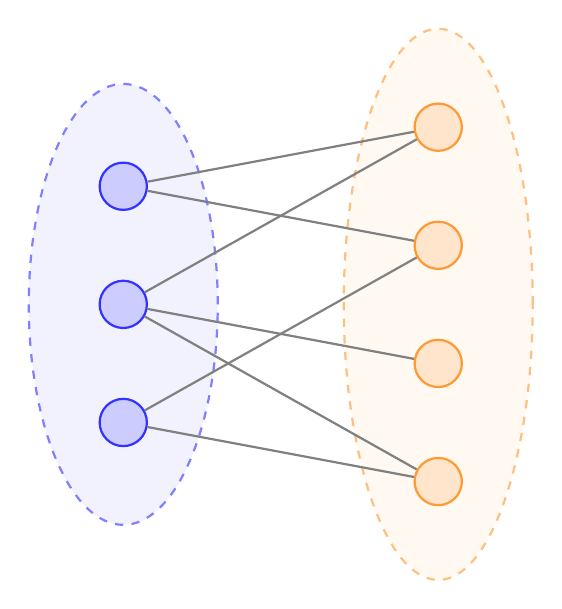
\begin{tikzpicture}[
    u-node/.style={circle, draw=blue!80, fill=blue!20, thick, minimum size=6mm},
    v-node/.style={circle, draw=orange!80, fill=orange!20, thick, minimum size=6mm},
    edge/.style={draw=black!50, thick}
]

    \draw[draw=blue!50, fill=blue!5, thick, dashed] (0,0) ellipse (1.2cm and 2.8cm);
    
    \draw[draw=orange!50, fill=orange!5, thick, dashed] (4,0) ellipse (1.2cm and 3.5cm);

    \node[u-node] (u1) at (0, 1.5) {};
    \node[u-node] (u2) at (0, 0) {};
    \node[u-node] (u3) at (0, -1.5) {};

    \node[v-node] (v1) at (4, 2.25) {};
    \node[v-node] (v2) at (4, 0.75) {};
    \node[v-node] (v3) at (4, -0.75) {};
    \node[v-node] (v4) at (4, -2.25) {};

    \draw[edge] (u1) -- (v1);
    \draw[edge] (u1) -- (v2);
    \draw[edge] (u2) -- (v1);
    \draw[edge] (u2) -- (v3);
    \draw[edge] (u2) -- (v4);
    \draw[edge] (u3) -- (v2);
    \draw[edge] (u3) -- (v4);

\end{tikzpicture}
\end{center}

See, this is a bipartite graph! Neither partition may contain internal edges.

They are often used in maximum bipartite matching, minimum vertex cover, and maximum independent set problems. They are equivalent by \emph{Kőnig's Theorem}:


\begin{mdquote}
    Let $G = (U \cup V, E)$ be a bipartite graph. Then:
    $$ |M_{\max}| = |C_{\min}| $$
    where $M_{\max}$ is a maximum matching and $C_{\min}$ is a minimum vertex cover.
\end{mdquote}


\begin{Question}{Hungarian Algorithm $\bigstar\bigstar$}
There are \texttt{m} boys and \texttt{n} girls in a class attending an upcoming party.

Given an $\texttt{m}\times\texttt{n}$ integer matrix \texttt{grid}, where \texttt{grid[i][j]} equals \texttt{0} or \texttt{1}. If \texttt{grid[i][j]==1}, then that means the $\texttt{i}^{\texttt{th}}$ boy can invite the $\texttt{j}^{\texttt{th}}$ girl to the party. A boy can invite at most one girl, and a girl can accept at most one invitation from a boy.

Return the maximum possible number of accepted invitations.
\end{Question}

The algorithm is straightforward and somewhat \emph{greedy} --- try the first available edge for each node in the left partition, and if a subsequent left node's desired right node is already occupied, backtrack to its current match to see if there are other possibilities. That's all there is to the \textbf{Hungarian Algorithm}.

\begin{lstlisting}[style=python]
class Solution:
    def match(self, grid: list[list[int]], l: int) -> bool:
        for r in range(self.n):
            if not grid[l][r] or self.visr[r]:
                continue
            self.visr[r] = True
            if r not in self.mapleft or self.match(grid, self.mapleft[r]):
                self.mapleft[r] = l
                return True
                
        return False

    def maximumInvitations(self, grid: list[list[int]]) -> int:
        self.m = len(grid)
        self.n = len(grid[0])
        self.mapleft = {}
        ans = 0
        
        for i in range(self.m):
            self.visr = [False] * self.n
            if self.match(grid, i):
                ans += 1
                
        return ans
\end{lstlisting}


\begin{Question}{Maximum Students Taking Exam $\bigstar\bigstar\bigstar$}
Given a $\texttt{m}\times\texttt{n}$ matrix \texttt{seats} that represent seats distributions in a classroom. If a seat is broken, it is denoted by \texttt{'\#'} character otherwise it is denoted by a \texttt{'.'} character.

Students can see the answers of those sitting next to the left, right, upper left and upper right, but he cannot see the answers of the student sitting directly in front or behind him. Return the maximum number of students that can take the exam together without any cheating being possible.
\end{Question}

This is, at first glance, a maximum independent set problem.

But what are the two partitions?

If we separate the odd columns and the even columns, they form a bipartite graph --- neither partition has internal edges, only edges connecting them. Each position can have \textbf{AT MOST} one person. Construct the graph by connecting those edges, then run the Hungarian Algorithm!

\newpage

\begin{lstlisting}[style=python]
class Solution:
    def check(self, seat: int, field: int) -> bool:
        sx, sy = self.pos[seat]
        fx, fy = self.pos[field]
        return abs(sx - fx) <= 1 and abs(sy - fy) == 1

    def match(self, seats: list[list[str]], l: int) -> bool:
        for r in self.graph[l]:
            if self.visr[r]:
                continue
            self.visr[r] = True
            if self.mapl[r] == -1 or self.match(seats, self.mapl[r]):
                self.mapl[r] = l
                return True
                
        return False

    def maxStudents(self, seats: list[list[str]]) -> int:
        self.m = len(seats)
        self.n = len(seats[0])
        self.pos = []
        
        for i in range(self.m):
            for j in range(self.n):
                if seats[i][j] == '.':
                    self.pos.append((i, j))
                    
        self.size = len(self.pos)
        self.graph = [list() for i in range(self.size)]
        self.mapl = [-1] * self.size
        self.visr = [False] * self.size
        
        for i in range(self.size):
            for j in range(self.size):
                if self.pos[i][1] % 2 == 0 and self.pos[j][1] % 2 == 1 and self.check(i, j):
                    self.graph[i].append(j)
                    
        cnt = 0
        
        for i in range(self.size):
            if self.pos[i][1] % 2 == 1:
                continue
            self.visr = [False] * self.size
            if self.match(seats, i):
                cnt += 1
                
        return self.size - cnt
\end{lstlisting}

\begin{Question}{Muddy Fields $\bigstar\bigstar\bigstar\bigstar$}
Given an $\texttt{m}\times\texttt{n}$ grid consisting of muddy cells \texttt{'*'} and grassy cells \texttt{'.'}, find the minimum number of wooden boards needed to cover all muddy cells.

Rules:
\begin{itemize}
    \item Each board has a width of \texttt{1} and any integer length.
    \item Boards can only be placed horizontally or vertically.
    \item Boards may overlap each other.
    \item Boards must not cover any grassy cells.
\end{itemize}
\end{Question}

This even looks NP-ish. But stay calm --- I put this question in this section, which implies it can be solved in polynomial time using a minimum vertex cover algorithm. Fortunately, we can!

Treat every muddy hole as an edge, and the two partitions as the horizontal and vertical wooden boards. After that, every muddy hole serves as an edge connecting a horizontal board to a vertical board. Think about a continuous line of mud that only has a width of 1: it would represent just one vertical board, but multiple length-1 horizontal boards. After that, the Hungarian Algorithm is all you need!

\begin{lstlisting}[style=python]
class Solution:
    def match(self, u: int) -> bool:
        for v in self.graph[u]:
            if self.vis[v]:
                continue
            self.vis[v] = True
            if self.matchV[v] == -1 or self.match(self.matchV[v]):
                self.matchV[v] = u
                return True
                
        return False

    def minBoards(self, grid: list[str]) -> int:
        if not grid or not grid[0]:
            return 0
        R = len(grid)
        C = len(grid[0])
        rowID = [[-1] * C for i in range(R)]
        colID = [[-1] * C for i in range(R)]
        uCnt = 0
        vCnt = 0
        
        for r in range(R):
            inSegment = False
            for c in range(C):
                if grid[r][c] == '*':
                    rowID[r][c] = uCnt
                    inSegment = True
                elif inSegment:
                    uCnt += 1
                    inSegment = False
            if inSegment: 
                uCnt += 1
                
        for c in range(C):
            inSegment = False
            for r in range(R):
                if grid[r][c] == '*':
                    colID[r][c] = vCnt
                    inSegment = True
                elif inSegment:
                    vCnt += 1
                    inSegment = False
            if inSegment: 
                vCnt += 1
                
        self.graph = [list() for i in range(uCnt)]
        
        for r in range(R):
            for c in range(C):
                if grid[r][c] == '*':
                    self.graph[rowID[r][c]].append(colID[r][c])
                    
        self.matchV = [-1] * vCnt
        ans = 0
        
        for u in range(uCnt):
            self.vis = [False] * vCnt
            if self.match(u):
                ans += 1
                
        return ans
\end{lstlisting}

\textbf{Note:} Beyond the Hungarian Algorithm, a more general approach is \emph{maximum flow} --- but I'm not going to go too deeply into this topic --- if you're interested, please take a look at \emph{Dinic's Algorithm}!




\newpage

\section{Algorithms}

\subsection{Handy Tricks}

\subsubsection{Prime Sieve}

\emph{Euler Sieve} is the most popular way to do this, and sieving is one of the first topics in number theory. How do we do it in $\mathcal O(n)$? Or in other words, how do we avoid counting the same number twice?

Intuitively, think of every composite number as a prime times something else. We can scan through all numbers and multiply each prime that is less than or equal to them, making sure the product is no larger than $n$.

\begin{lstlisting}[style=python]
for i in range(2, n + 1):
    for p in primes:
        if i * p > n:
            break
        is_prime[i * p] = False
\end{lstlisting}

However, this is not $\mathcal O(n)$ (think about $4\times3$ and $6\times2$) --- anyways, we've invented \emph{Eratosthenes Sieve}! Actually, the Euler Sieve merely adds \textbf{ONE} conditional line to handle this rule, that is, to skip those divisibility conditions.

\begin{lstlisting}[style=python]
res = 1
while b > 0:
    if b % 2 == 1:
        res = res * a
    a = a * a
    b = b // 2
\end{lstlisting}

\subsubsection{KMP Algorithm}

\emph{Knuth-Morris-Pratt Algorithm} is the classical deterministic way to match strings, though nowadays search engines are not likely to use it. It is a method for matching an $\mathcal O(m)$ target string within a large $\mathcal O(n)$ source text and returning its location in $\mathcal O(m+n)$ time. It is the optimal lower bound.

Let's think about a middle step --- suppose we are trying to match \texttt{ABAC} using pointer \texttt{p1} within the string \texttt{ABABAC} using pointer \texttt{p2}. Right now, \texttt{p1} is at \texttt{C} and \texttt{p2} is at the second \texttt{B}. It looks like they don't match, but we don't reset \texttt{p2} to the first \texttt{B} this time. Instead, we keep \texttt{p2} stable and move \texttt{p1} to the nearest prefix re-match (\texttt{p1} can even jump further back after this, if needed, which is doable in $\mathcal{O}(m)$ time). So \texttt{p1} becomes \texttt{B} again, and then the whole string matches!

Technically, whenever we find a letter that does not match, \texttt{p1} jumps by checking the longest, then the second longest, maximum common prefix-suffix of the substring before it. Note that this can jump at most $\mathcal O(n)$ times in total, which is exactly the intuition behind \emph{Amortized Analysis}.

\begin{lstlisting}[style=python]
j = 0
for i in range(1, m):
    while j > 0 and pattern[i] != pattern[j]:
        j = next_arr[j - 1]
    if pattern[i] == pattern[j]:
        j += 1
    next_arr[i] = j
j = 0
for i in range(n):
    while j > 0 and text[i] != pattern[j]:
        j = next_arr[j - 1]
    if text[i] == pattern[j]:
        j += 1
    if j == m:
        return i - m + 1
\end{lstlisting}


\subsubsection{Quick Power}

\emph{Quick Power} is another small and handy trick that gives us some food for thought.

The power $2^{10}$ is the same as $2^{(1010)_2} = 2^8 \times 2^2$, we only need $\mathcal O(\log n)$ time to calculate $2^1, 2^2, 2^4, \dots$, and that's enough!

\begin{lstlisting}[style=python]
res = 1
while b > 0:
    if b % 2 == 1:
        res = res * a
    a = a * a
    b = b // 2
\end{lstlisting}

What if the exponent is unprecedentedly large? Check \emph{Extended Euler's Theorem} or \emph{Lightspeed Power} in $\mathcal O(1)$ time!

\begin{Question}{Lightspeed Power $\bigstar\bigstar\bigstar$}
Given fixed base \texttt{a} and fixed modulo \texttt{mod}, compute $\texttt{a}^{\texttt{b}}\ \texttt{(mod)}$ for $\texttt{10}^{\texttt{7}}$ queries, where the exponent $\texttt{b}$ is within a \texttt{32-bit} integer range.

\end{Question}

The core idea is:

$$
a^b=a^{x\times S}\times a^y
$$

where we often choose $S=\sqrt{n}$, which in this case is $2^{16}$.

\begin{lstlisting}[style=python]
pow1 = [0] * 65536
pow2 = [0] * 65536

def preproc():
    pow1[0] = 1
    pow2[0] = 1
    
    for i in range(1, 65536):
        pow1[i] = (pow1[i - 1] * a) % mod
        
    pow65536 = (pow1[65535] * a) % mod
    
    for i in range(1, 65536):
        pow2[i] = (pow2[i - 1] * pow65536) % mod
def query(pows):
    return (pow1[pows & 65535] * pow2[pows >> 16]) % mod
\end{lstlisting}


\subsection{Search}

\subsubsection{DFS}

\textbf{Depth-First} uses \textbf{LIFO}, it has the following template:

\begin{lstlisting}[style=python]
def dfs(node):
    if node in visited:
        return
    visited.add(node)
    for nxt in node.nexts:
        dfs(nxt)
\end{lstlisting}

Set \texttt{visited} ensures that we never visit the same node twice. This runs in $\mathcal{O}(V+E)$ time.

\begin{Question}{Sum of Root To Leaf
 $\bigstar$}
Given the \texttt{root} of a binary tree where each node has a value \texttt{0} or \texttt{1}. Each root-to-leaf path represents a binary number starting with the most significant bit.

\begin{itemize}
    \item For example, if the path is \texttt{0->1->1->0->1}, then this could represent \texttt{01101} in binary, which is \texttt{13}.
\end{itemize}

For all leaves in the tree, consider the numbers represented by the path from the root to that leaf. Return the sum of these numbers.
\end{Question}

Think of the data stream as starting from the root (top to bottom), passing to each child, and concluding the answer after all paths have been processed.

\begin{lstlisting}[style=python]
class Solution:
    def sumRootToLeaf(self, root: Optional[TreeNode]) -> int:
        def dfs(node, val) -> int:
            if not node: return 0
            val = (val << 1) | node.val
            if not node.left and not node.right: return val
            return dfs(node.left, val) + dfs(node.right, val)
            
        return dfs(root, 0)
\end{lstlisting}

\begin{Question}{Lowest Common Ancestor
 $\bigstar$$\bigstar$}
Given the \texttt{root} of a binary tree, return the lowest common ancestor of its deepest leaves.
\end{Question}

We need to know the depth of every node to determine the LCA. So, perform a bottom-up DFS this time. It has a \emph{Tree Divide and Conquer} idea behind it.

\begin{lstlisting}[style=python]
class Solution:
    def lcaDeepestLeaves(self, root: Optional[TreeNode]) -> Optional[TreeNode]:
        def dfs(node, depth) -> tuple[TreeNode, int]:
            ldepth = depth
            rdepth = depth
            if node.left:
                lnode, ldepth = dfs(node.left, depth + 1)
            if node.right:
                rnode, rdepth = dfs(node.right, depth + 1)
            if ldepth > rdepth:
                return lnode, ldepth
            elif ldepth < rdepth:
                return rnode, rdepth
            else:
                return node, ldepth
                
        ans, _ = dfs(root, 0)
        return ans
\end{lstlisting}

\textbf{Note:} If we are supposed to find all possible paths, DFS can perform a special technique: \emph{backtracking}. This runs in exponential time.

\begin{lstlisting}[style=python]
def dfs(node):
    if node in visited:
        return
    visited.add(node)
    for nxt in node.nexts:
        dfs(nxt)
    visited.remove(node)
\end{lstlisting}

\subsubsection{BFS}

\textbf{Breadth-First} uses \textbf{FIFO}, it has the following template:

\begin{lstlisting}[style=python]
while queue:
    node = queue.popleft()
    for nxt in node.nexts:
        if nxt not in visited:
            visited.add(nxt)
            queue.append(nxt)
\end{lstlisting}

This also runs in $\mathcal{O}(V+E)$ time, with higher memory consumption than DFS.

For interval search spaces, the common BFS is $\mathcal{O}(n^2)$, but this can be improved to $\mathcal{O}(n\log n)$ using a red-black tree or $\mathcal{O}(n\alpha(n))$ using Jump DSU (recommended, see an earlier question).

\subsubsection{Binary Search}

Python provides binary search functions:

\begin{lstlisting}[style=python]
lower_bound = bisect.bisect_left(arr, target)
upper_bound = bisect.bisect_right(arr, target)
\end{lstlisting}

If we need to do more than simply find the bisect position, we'll need to write binary search by hand.

\begin{Question}{Eating Bananas $\bigstar$}
There are \texttt{n} piles of bananas, the $\texttt{i}^{\texttt{th}}$ pile has \texttt{piles[i]} bananas. The guards have gone and will come back in \texttt{h} hours.

The monkey can decide its bananas-per-hour eating speed of \texttt{k}. Each hour, it chooses some pile of bananas and eats \texttt{k} bananas from that pile. If the pile has less than \texttt{k} bananas, it eats all of them instead and will not eat any more bananas during this hour.

The monkey likes to eat slowly but still wants to finish eating all the bananas before the guards return.

Return the minimum integer \texttt{k} such that the monkey can eat all the bananas within \texttt{h} hours.
\end{Question}

\begin{lstlisting}[style=python]
class Solution:
    def minEatingSpeed(self, piles: list[int], h: int) -> int:
        piles.sort()
        n = len(piles)
        l = 1
        r = piles[n - 1]
        
        while l < r:
            mid = l + (r - l) // 2
            if self.check(piles, h, mid):
                r = mid
            else:
                l = mid + 1
                
        return r

    def check(self, piles: list[int], h: int, k: int) -> bool:
        time = 0
        
        for i in piles:
            time += math.ceil(i / k)    
            
        if time <= h:
            return True
        return False
\end{lstlisting}

\subsection{Divide and Conquer}

There is another special word for \textbf{Divide and Conquer} --- \emph{non-overlapping substructures}.

Segment trees (see before) and Merge Sort are typical examples of \textbf{Classical D\&C}. Besides these, \textbf{Tree D\&C} is another big branch (known as \emph{Centroid Decomposition} and \emph{Edge Decomposition}).

\begin{Question}{2-Merge Sort $\bigstar$}
Given the heads of two sorted linked lists \texttt{list1} and \texttt{list2}.

Merge the two lists into one sorted list. The list should be made by splicing together the nodes of the first two lists.
\end{Question}

Consider two pointers \texttt{p1} and \texttt{p2} for \texttt{list1} and \texttt{list2}. Since they are pre-sorted, the only work left is to compare \texttt{*p1} and \texttt{*p2} each time before deciding which pointer to move right!

\begin{lstlisting}[style=python]
class Solution:
    def mergeTwoLists(self, list1: Optional[ListNode], list2: Optional[ListNode]) -> Optional[ListNode]:
        root = ListNode(-1)
        current = root
        
        while list1 and list2:
            if list1.val < list2.val:
                current.next = list1
                list1 = list1.next
            else:
                current.next = list2
                list2 = list2.next
            current = current.next
            
        if list1:
            current.next = list1
        if list2:
            current.next = list2
        return root.next
\end{lstlisting}


\begin{Question}{k-Merge Sort $\bigstar$$\bigstar$}
Given an array of \texttt{k} linked-lists \texttt{lists}, each linked-list is sorted in ascending order.

Merge all the linked-lists into one sorted linked-list and return it.
\end{Question}

If we follow the same procedure, the difference here is how to compare $k$ numbers to decide which pointer to move (which could easily go up to $\mathcal O(nk)$ time)! So, time to use a min-heap again, with a time complexity of $\mathcal O(n\log k)$.

\begin{lstlisting}[style=python]
class Solution:
    def mergeKLists(self, lists: List[Optional[ListNode]]) -> Optional[ListNode]:
        root = ListNode(-1)
        current = root
        heap = []
        
        for i, node in enumerate(lists):
            if node:
                heapq.heappush(heap, (node.val, i, node))
                
        while heap:
            val, i, node = heapq.heappop(heap)
            current.next = node
            current = current.next
            if node.next:
                heapq.heappush(heap, (node.next.val, i, node.next))
                
        return root.next
\end{lstlisting}



\subsection{Dynamic Programming}

There is another special word for \textbf{Dynamic Programming} --- \emph{overlapping substructures}.

\textbf{Note:} We are mostly implementing DP in a \emph{bottom-up} way rather than \emph{top-down / memoization} below. I like DP ideas very much at least when writing this.

Let's explore some classical examples of \textbf{Linear DP} at the beginning.

\textbf{a) Linear DP}

\textbf{Longest Increasing Subsequence} --- given a sequence $L$, find the length of the longest subsequence in which all elements are strictly increasing:

$$
f(i)=
\begin{cases}
1, & n(i) \le n(i-k) \\
\displaystyle\max_k f(i-k)+1, & n(i)>n(i-k)
\end{cases}
$$

where $f(i)$ represents the length of the longest increasing subsequence ending at index $i$.

\textbf{Longest Increasing Subarray} --- the difference is subtle again: 

$$
f(i)=
\begin{cases}
1, & n(i) \le n(i-1) \\
f(i-1)+1, & n(i)>n(i-1)
\end{cases}
$$

\textbf{Longest Common Subsequence} --- for sequence $p$ with length $m$ and sequence $q$ with length $n$:

$$
f(i,j)=
\begin{cases}
\max(f(i-1,j),f(i,j-1)), & p(i)\neq q(j) \\
f(i-1,j-1)+1, & p(i)=q(j)
\end{cases}
$$

where $f(i,j)$ represents the length of the longest common subsequence between $p[0...i]$ and $q[0...j]$.

\textbf{Maximum Subarray Sum} --- given an integer array a, find the contiguous subarray with the largest possible sum and return that sum:

$$
f(i)=\max(f(i-1)+a(i),a(i))
$$

where $i$ represents the last index of the subarray with the maximum sum ending at $i$. This is also known as \emph{Kadane's Algorithm}.

\textbf{Gap-Taxed Largest Subsequence} --- we introduce a penalty when there is a gap between two selected elements. For example, define the tax as:

$$
\text{penalty}(i,j)=(i-j-1)^2
$$

then the state transition becomes:

$$
f(i)=\max_{j<i}\left(a(i), f(j)+a(i)-\text{penalty}(i,j)\right)
$$

where $f(i)$ represents the maximum score of a gap-taxed subsequence ending at index $i$. This can be viewed as a generalization of \emph{Kadane's Algorithm}.

\emph{Knapsack DP} is a huge branch of Linear DP. Now let's take a closer look at it.

\textbf{0/1 Knapsack} --- given a set of $n$ items, where each item has a weight $w_i$ and a value $v_i$, the goal is to select the most valuable subset of items that fits within a knapsack of capacity $W$.

This is also known as the \emph{yes/no choice} pattern: for each item, we either take it or leave it.

The substructure is built at item step $i$:

$$
f(i,W)=\max(f(i-1,W),f(i-1,W-w(i))+v(i))
$$

where $f(0,W)=0$ and $i=1,2,\dots,n$.

\textbf{Fractional Knapsack} --- we can take fractional items, it can be solved by a \emph{Greedy Algorithm}.

\textbf{Bounded/Unbounded Knapsack} --- the tiny difference here is whether each item has a limited number of copies. Bounded means each item has a fixed limit (also called \textbf{Multiple Knapsack}), while unbounded means we can take unlimited copies (also called \textbf{Complete Knapsack}).

For the unbounded case:

$$
f(i,W)=\max(f(i-1,W),f(i,W-w(i))+v(i))
$$

where $i$ represents the current item type.

For the bounded case:

$$
f(i,W)=\max_{0\leq k\leq k_i}(f(i-1,W-kw(i))+kv(i))
$$

where $k_i$ is the maximum number of copies allowed for item $i$.

\textbf{Multi-dimensional Knapsack} --- the formulation is:

$$
\max \sum_{i=1}^n v_ix_i
\quad \text{S.T.}\quad
\sum_{i=1}^n w_{ij}x_i\leq W_j
$$

where $x_i\in\{0,1\}$.

The recurrence is quite similar (but in vectors):

$$
f(i,\boldsymbol W)=\max(f(i-1,\boldsymbol W),f(i-1,\boldsymbol W-\boldsymbol w(i))+v(i))
$$

this is getting insanely expensive as the dimension grows, so it is often combined with other techniques for pruning.


The complexity above is determined by the size of the DP matrix, which is $\mathcal O(nW)$ for the one-dimensional case, or $\mathcal O(nW_1\cdots W_d)$ for the multi-dimensional case.

\textbf{Note:} I believe this is enough for Linear DP exercises, and please take some time to digest them!



And one more thing --- AI is everywhere, and I feel it is important to show DP in \textbf{Backpropagation}:

\emph{You are given a multilayer neural network with $M$ layers and $N$ neurons per layer.}

\emph{For each layer $i$:}

\begin{itemize}
    \item \emph{$a^i_j$: the output representation of neuron $j$ in layer $i$}
    \item \emph{$w^i_{j,k}$: the weight connecting neuron $j$ in layer $i$ to neuron $k$ in layer $i+1$}
    \item \emph{$f(\cdot)$: the activation function}
    \item \emph{$\ell$: the final loss}
\end{itemize}

\emph{The task is to compute:}

$$
\frac{\partial \ell}{\partial w^i_{j,k}}
$$

\emph{in $\mathcal O(MN^2)$ time.}

The key idea is simple --- we reuse intermediate gradients through dynamic programming:

$$
\frac{\partial z}{\partial a^i_j}
=
\sum_{k=1}^{N}
\frac{\partial z}{\partial a^{i+1}_k}
\cdot
\frac{\partial a^{i+1}_k}{\partial a^i_j}
$$

$$
\frac{\partial z}{\partial w^i_{j,k}}
=
\sum_{m=1}^{N}
\frac{\partial z}{\partial a^i_m}
\cdot
\frac{\partial a^i_m}{\partial w^i_{j,k}}
$$

where $i$ denotes the $i^{\text{th}}$ layer, $a^i$ represents the hidden representation of layer $i$, $w^i_{j,k}$ is the $(j,k)^{\text{th}}$ entry of the weight matrix at layer $i$, and $z$ represents the loss function.






\textbf{b) Interval DP}

Let's start with my favorite classical palindrome problems.

\begin{Question}{Longest Palindromic Subsequence
 $\bigstar$$\bigstar$}
Given a string \texttt{s}, find the longest palindromic subsequence's length in \texttt{s}.

A subsequence is a sequence that can be derived from another sequence by deleting some or no elements without changing the order of the remaining elements.
\end{Question}

For a \emph{palindrome}, the intuition is to consider two directions, i.e. going left and going right.

So use a 2D DP array to store the lengths, where the two dimensions represent the start and end indices of the string respectively. The state transition is, if the characters at both ends are equal, \texttt{dp[i][j] = dp[i+1][j-1] + 2}, plus the boundary condition for \texttt{j-i <= 1}.

Otherwise, run \texttt{dp[i][j] = max(dp[i+1][j],dp[i][j-1])}.

\begin{lstlisting}[style=python]
class Solution:
    def longestPalindromeSubseq(self, s: str) -> int:
        n = len(s)
        dp = [[0] * n for _ in range(n)]
        
        for i in range(n - 1, -1, -1):
            dp[i][i] = 1 
            for j in range(i + 1, n):
                if s[i] == s[j]:
                    dp[i][j] = dp[i + 1][j - 1] + 2
                else:
                    dp[i][j] = max(dp[i + 1][j], dp[i][j - 1])
                    
        return dp[0][n - 1]
\end{lstlisting}

Hold on! Think again about a subtle property here. We know that a subsequence doesn't have to be contiguous, so the state transition follows an additive rule, i.e. an inner result can contribute directly to its enclosing interval. But what if, the subsequence has to be contiguous? What happens then?

\begin{Question}{Longest Palindromic Substring
 $\bigstar$$\bigstar$}
Given a string \texttt{s}, return the longest palindromic substring in \texttt{s}.
\end{Question}

The additive rule doesn't apply here. We can't simply use \texttt{dp[i][j] = dp[i+1][j-1] + 2} for the state transition anymore. So what's left? We can only mark each substring with a boolean indicating whether it's a palindrome, and maintain a global counter as we go.

\begin{lstlisting}[style=python]
class Solution:
    def longestPalindrome(self, s: str) -> str:
        n = len(s)
        dp = [[False] * n for _ in range(n)]
        ans, idx = 0, -1
        
        for l in range(1, n + 1):
            for i in range(n - l + 1):
                j = i + l - 1
                if j >= n: break
                if s[i] == s[j]:
                    if j - i <= 1: dp[i][j] = True
                    else: dp[i][j] = dp[i + 1][j - 1]
                if dp[i][j] and ans < j - i + 1:
                    ans = j - i + 1
                    idx = i
                    
        return s[idx:idx + ans]
\end{lstlisting}

We might find it often to define \texttt{i} and \texttt{j} as the start and end indices of a string. But note that \textbf{NOT} all 2D arrays are \textbf{Interval DP}s, since they should have two indices representing directions on the same measure.

\begin{Question}{Zuma
 $\bigstar$$\bigstar$$\bigstar$}
Genos recently installed the game Zuma on his phone. In Zuma there exists a line of $\texttt n$ gemstones, the $\texttt{i}^{\texttt{th}}$ of which has color $\texttt{c}_{\texttt{i}}$. The goal of the game is to destroy all the gemstones in the line as quickly as possible.

In one second, Genos is able to choose exactly one continuous substring of colored gemstones that is a palindrome and remove it from the line. After the substring is removed, the remaining gemstones shift to form a solid line again. What is the minimum number of seconds needed to destroy the entire line?
\end{Question}

Can we use a \emph{Greedy Algorithm} here? Unfortunately, it doesn't always work (think about why \texttt{1,2,1,1,3,1}). By this counterexample, the time complexity rises to $\mathcal O(n^3)$:

$$
f(i,j) = \begin{cases} 
\min \begin{cases} 
f(i+1,j-1) \\ 
\displaystyle\min_k (f(i,k)+f(k+1,j)) 
\end{cases}, & \text{if colors}[i] == \text{colors}[j] \\ 
\displaystyle\min_k (f(i,k)+f(k+1,j)), & \text{if colors}[i] \neq \text{colors}[j] 
\end{cases}
$$

which has a shrinking algorithm and a splitting algorithm.

\begin{lstlisting}[style=python]
class Solution:
    def minimumMoves(self, colors: List[int]) -> int:
        n = len(colors)
        if n == 0:
            return 0
        dp = [[float('inf')] * n for _ in range(n)]
        
        for length in range(1, n + 1):
            for i in range(n):
                j = i + length - 1
                if j >= n:
                    break
                if i == j:
                    dp[i][j] = 1
                    continue
                if colors[i] == colors[j]:
                    if j - i == 1:
                        dp[i][j] = 1
                    else:
                        dp[i][j] = dp[i + 1][j - 1]
                for k in range(i, j):
                    dp[i][j] = min(dp[i][j], dp[i][k] + dp[k + 1][j])
                    
        return dp[0][n - 1]
\end{lstlisting}


\textbf{c) Tree DP}

As the name suggests, \textbf{Tree DP} is simply DP on a tree.

\begin{Question}{House Robber
 $\bigstar$$\bigstar$}
The thief has found himself a new place for his thievery again. There is only one entrance to this area, called \texttt{root}.

Besides the \texttt{root}, each house has one and only one parent house. After a tour, the smart thief realized that all houses in this place form a binary tree. It will automatically contact the police if two directly-linked houses were broken into on the same night.

Given the \texttt{root} of the binary tree, return the maximum amount of money the thief can rob without alerting the police.
\end{Question}

This problem is very suitable for overlapping substructures.

\newpage

Think about:

$$f(u) = \max \begin{cases} \text{val}(u) + \displaystyle\sum_{v \in \text{grandchild}(u)} f(v), & \text{(if steal } u) \\ \displaystyle\sum_{v \in \text{child}(u)} f(v), & \text{(if not steal } u). \end{cases}$$

\begin{lstlisting}[style=python]
class Solution:
    def rob(self, root: Optional[TreeNode]) -> int:
        def dp(node) -> tuple[int, int]:
            if not node:
                return (0, 0)
            ly, ln = dp(node.left)
            ry, rn = dp(node.right)
            return (node.val + ln + rn, max(ly, ln) + max(ry, rn))
            
        ry, rn = dp(root)
        return max(ry, rn)
\end{lstlisting}




\begin{Question}{Binary Tree Maximum Path Sum
 $\bigstar$$\bigstar$}
A path in a binary tree is a sequence of nodes where each pair of adjacent nodes in the sequence has an edge connecting them. A node can only appear in the sequence at most once. Note that the path does not need to pass through the root.

The path sum of a path is the sum of the node's values in the path.

Given the \texttt{root} of a binary tree, return the maximum path sum of any non-empty path.
\end{Question}

The question needs a translation before solving. Think about it: every path should have one and only one root, so let's store the maximum straight path sum for every node. The answer would be obtained by adding two subtrees together and comparing them:

$$f(u) = \max_{v \in \text{child}(u)} g(v).$$

\begin{lstlisting}[style=python]
class Solution:
    def maxPathSum(self, root: Optional[TreeNode]) -> int:
        ans = -1000 
        
        def dp(node) -> int:
            nonlocal ans
            if not node:
                return 0
            l = dp(node.left)
            r = dp(node.right)
            ans = max(ans, node.val + max(0, l) + max(0, r))
            return node.val + max(0, l, r)
            
        dp(root)
        return ans
\end{lstlisting}

\textbf{d) Bitmask DP}

\textbf{Bitmask DP} is a special branch of DP. Its core idea is to use a bit number to represent a state.

\begin{Question}{Held-Karp Algorithm
 $\bigstar$$\bigstar$$\bigstar$$\bigstar$}
Given an array of strings \texttt{words}, return the smallest string that contains each string in \texttt{words} as a substring. If there are multiple valid strings of the smallest length, return any of them.

May assume that no string in \texttt{words} is a substring of another string in \texttt{words}.
\end{Question}

It's common for a word's suffix to overlap with another word's prefix --- how do we count this (or modelize this)? Here comes the first Aha moment: define \texttt{w(i,j)} to represent the overlap between the \texttt{i-suffix} and the \texttt{j-prefix} (the graph is directional).

Now the problem is translated into: for a weighted directed graph, how do we find the shortest path that connects all of them?

The first intuition is to split any connected edge in $S$ and add a $v\notin S$ to insert into one of them, before deleting the longest edge. However, it's easy to see that this will result in disconnected components. We need to make sure that the previous path wouldn't be cut!

Here comes the second Aha moment by applying Bitmask DP:

$$f(S \cup \{v\}, v) = f(S, u) + w(u, v)$$

where $u$ is the last node of $S$.

The second step is also called the \emph{Travelling Salesman Problem (TSP)}, which is one of the most famous NP-complete problems. We have $\mathcal O(2^n)$ for enumerating $S$, and $\mathcal O(n)$ for checking whether $v$ is outside $S$, and we count $\mathcal O(n)$ times for every u∈S, so the complexity is $\mathcal O(n^22^n)$.

\begin{lstlisting}[style=python]
class Solution:
    def shortestSuperstring(self, words: List[str]) -> str:
        n = len(words)
        w = [[0] * n for _ in range(n)]
        
        for i in range(n):
            for j in range(n):
                if i != j:
                    max_overlap = 0
                    min_len = min(len(words[i]), len(words[j]))
                    for k in range(min_len, 0, -1):
                        if words[i].endswith(words[j][:k]):
                            max_overlap = k
                            break
                    w[i][j] = len(words[j]) - max_overlap
                    
        dp = [[float('inf')] * n for _ in range(1 << n)]
        parent = [[-1] * n for _ in range(1 << n)]
        
        for i in range(n):
            dp[1 << i][i] = len(words[i])
            
        for S in range(1, 1 << n):
            for i in range(n):
                if not (S & (1 << i)): continue
                for j in range(n):
                    if S & (1 << j): continue 
                    next_S = S | (1 << j)
                    if dp[S][i] + w[i][j] < dp[next_S][j]:
                        dp[next_S][j] = dp[S][i] + w[i][j]
                        parent[next_S][j] = i
                        
        final_state = (1 << n) - 1
        min_len = float('inf')
        last_node = -1
        
        for i in range(n):
            if dp[final_state][i] < min_len:
                min_len = dp[final_state][i]
                last_node = i
        path = []
        curr_state = final_state
        curr_node = last_node
        
        while curr_node != -1:
            path.append(curr_node)
            prev_node = parent[curr_state][curr_node]
            curr_state ^= (1 << curr_node)
            curr_node = prev_node
            
        path.reverse()
        ans = words[path[0]]
        
        for i in range(1, len(path)):
            prev_word = path[i-1]
            curr_word = path[i]
            cost = w[prev_word][curr_word]
            if cost > 0:
                ans += words[curr_word][-cost:]
                
        return ans
\end{lstlisting}


\subsection{Graph Theory}

\subsubsection{Minimum Spanning Tree}

\textbf{Minimum Spanning Tree (MST)} algorithms are \emph{Greedy Algorithms}, based on the \emph{Cut Property}:

\begin{mdquote}
Let $G = (V, E)$ be a connected undirected graph with an edge weight function $w$, and let $S \subset V$ be any non-empty proper subset of vertices. Then:$$e = \arg\min_{e' \in \delta(S)} w(e') \implies e \in T$$where $\delta(S)$ is the set of edges crossing the cut $(S, V \setminus S)$, and $T$ is some minimum spanning tree of $G$.
\end{mdquote}

\textbf{a) Kruskal's Algorithm}

We use DSUs to implement Kruskal's Algorithm (and treat every node as a disjoint set at the beginning). For every edge connecting two different sets, pick it if it has the minimum weight, and iterate. The time complexity is $\mathcal O(E\log E)$. Looks like we are encountering more named algorithms!

\begin{lstlisting}[style=python]
def kruskal(all_nodes, all_edges):
    mst_edges = []
    
    for node in all_nodes:
        parent[node] = node
        
    sorted_edges = sorted(all_edges, key=lambda e: e.weight)
    
    for edge in sorted_edges:
        if union(edge.u, edge.v):
            mst_edges.append(edge)
            if len(mst_edges) == len(all_nodes) - 1:
                break
    
    return mst_edges
\end{lstlisting}


\textbf{b) Prim's Algorithm}

Prim's Algorithm is based on maintaining $V\setminus S$, and each time picking the smallest edge between $S$ and $V\setminus S$ to join in, often using a heap to maintain the order. The time complexity is $\mathcal O((V+E)\log V)$.

\begin{lstlisting}[style=python]
def prim(start_node):
    visited.add(start_node)
    for edge in start_node.edges:
        heapq.heappush(min_heap, (edge.weight, edge.to_node, edge))
        
    while min_heap:
        weight, next_node, current_edge = heapq.heappop(min_heap)
        if next_node in visited:
            continue
        visited.add(next_node)
        mst_edges.append(current_edge)
        for edge in next_node.edges:
            if edge.to_node not in visited:
                heapq.heappush(min_heap, (edge.weight, edge.to_node, edge))
                
    return mst_edges
\end{lstlisting}

\subsubsection{Single Source Shortest Path}

\textbf{Single Source Shortest Path (SSSP)} is probably the most classical problem in graph theory.

\textbf{a) Floyd-Warshall Algorithm}

Technically, Floyd-Warshall Algorithm is not single-sourced, it calculates all-pairs shortest paths using:

$$
f(i,j)=\min(f(i,j),f(i,k) + f(k,j)).
$$

The time complexity is $\mathcal O(V^3)$.

\begin{lstlisting}[style=python]
def floyd_warshall(all_nodes, dist_matrix):
    for k in all_nodes:
        for i in all_nodes:
            for j in all_nodes:
                if dist_matrix[i][k] + dist_matrix[k][j] < dist_matrix[i][j]:
                    dist_matrix[i][j] = dist_matrix[i][k] + dist_matrix[k][j]
\end{lstlisting}

\textbf{b) Dijkstra's Algorithm}

Dijkstra's Algorithm is a \emph{Greedy Algorithm} too (very much like Prim's Algorithm). The core idea is maintaining a visited set, and each time selecting the shortest edge between the set and the unvisited nodes (often using a min-heap here) and then we don't check it anymore. The time complexity is also $\mathcal O((V+E)\log V)$.

\textbf{Note:} It only works for graphs with non-negative edge weights.

\begin{lstlisting}[style=python]
def dijkstra(start_node, all_nodes):
    for node in all_nodes:
        dist[node] = float('inf')
    dist[start_node] = 0
    min_heap = [(0, start_node)]
    
    while min_heap:
        current_dist, current_node = heapq.heappop(min_heap)
        if current_dist > dist[current_node]:
            continue
        for edge in current_node.edges:
            neighbor = edge.to_node
            new_path_dist = current_dist + edge.weight
            if new_path_dist < dist[neighbor]:
                dist[neighbor] = new_path_dist
                heapq.heappush(min_heap, (new_path_dist, neighbor))
\end{lstlisting}

\textbf{c) Bellman-Ford Algorithm}

Bellman-Ford Algorithm could be used for finding negative-weight shortest paths. The time complexity is $\mathcal O(V\times E)$ based on the following \emph{Graph DP} transition:

$$
f(v)=\min(f(v),w(u,v)+f(u)).
$$

\begin{lstlisting}[style=python]
def bellman_ford(start_node, all_nodes, all_edges):
    for node in all_nodes:
        dist[node] = float('inf')
        
    dist[start_node] = 0
    V = len(all_nodes)
    
    for _ in range(V - 1):
        updated = False
        for edge in all_edges:
            u = edge.from_node
            v = edge.to_node
            if dist[u] + edge.weight < dist[v]:
                dist[v] = dist[u] + edge.weight
                updated = True
        if not updated:
            break
            
    return dist
\end{lstlisting}

\subsubsection{Strongly Connected Components}

\textbf{Strongly Connected Components (SCC)} are defined as components where every node can reach every other node in a directed graph. They are used to convert a directed graph into a \emph{Directed Acyclic Graph (DAG)}.

\textbf{a) Tarjan's Algorithm}

The key idea of Tarjan's Algorithm is the DFS number and the low-link value, based on three node states: unvisited, visited and in the stack, and visited but not in the stack. The nodes popped out at the same time form one complete SCC. The time complexity is $\mathcal O(V+E)$.

\textbf{Note:} For undirected graphs, DFS is enough for finding connected components. There is also Tarjan's Algorithm, which is used for finding \emph{Biconnected Components}.


\begin{lstlisting}[style=python]
def dfs(node):
    global time
    dfn[node] = time
    low[node] = time
    time += 1
    stack.append(node)
    on_stack.add(node)
    
    for nxt in node.nexts:
        if nxt not in dfn:
            dfs(nxt)
            low[node] = min(low[node], low[nxt])
        elif nxt in on_stack:
            low[node] = min(low[node], dfn[nxt])
    if low[node] == dfn[node]:
        scc = []
        while True:
            top = stack.pop()
            on_stack.remove(top)
            scc.append(top)
            if top == node:
                break
        all_sccs.append(scc)

def find_all_sccs(all_nodes):
    for node in all_nodes:
        if node not in dfn:
            dfs(node)
    return all_sccs
\end{lstlisting}


\textbf{b) Kosaraju's Algorithm}

Kosaraju's Algorithm applies a simple rule: the transpose of a directed graph does not change its SCCs (and only its SCCs). Note that the \emph{topological order} of the SCC stack never changes, even if the starting point of the DFS changes.

So --- if we perform a reverse DFS from the top of the topological stack, it ensures that each search really finds one SCC (instead of the circumstance where nodes that are not an SCC in the original graph appear to be connected in the transposed graph). The time complexity is $\mathcal O(V+E)$.

This idea is based on \emph{Topological Sort}.

\begin{lstlisting}[style=python]
def dfs_pass1(node):
    if node in visited:
        return
    visited.add(node)
    for nxt in node.nexts:
        dfs_pass1(nxt)
    stack.append(node)
    
def dfs_pass2(node):
    if node in visited:
        return
    visited.add(node)
    current_scc.append(node)
    for nxt in node.reversed_nexts:
        dfs_pass2(nxt)

def find_all_sccs(all_nodes):
    global current_scc
    
    for node in all_nodes:
        if node not in visited:
            dfs_pass1(node)
            
    visited.clear()
    
    while stack:
        node = stack.pop()
        if node not in visited:
            current_scc = []
            dfs_pass2(node)
            all_sccs.append(current_scc)
            
    return all_sccs
\end{lstlisting}


\subsubsection{Topological Sort}

\textbf{Topological Sort} is only defined on DAGs. This can also be used to check whether a cycle exists.

\textbf{a) DFS}

The first DFS pass in Kosaraju's Algorithm is a Topological Sort. The most magical thing here is that a single DFS stack contains all the information needed for the topological order --- source nodes must be on the top of the stack, and sink nodes must be at the bottom of the hierarchy. The time complexity is $\mathcal O(V+E)$.

\begin{lstlisting}[style=python]
def dfs_topo(node):
    if node in visiting:
        return False
    if node in visited:
        return True
    visiting.add(node)
    
    for nxt in node.nexts:
        if not dfs_topo(nxt):
            return False
            
    visiting.remove(node)
    visited.add(node)
    stack.append(node)
    return True

def dfs_topological_sort(all_nodes):
    for node in all_nodes:
        if node not in visited:
            if not dfs_topo(node):
                return None
                
    return stack[::-1]
\end{lstlisting}


\textbf{b) Kahn's Algorithm}

Kahn's Algorithm is using a queue to store all 0-in-degree nodes. For each turn, remove them and update the in-degrees, resulting in the topological order (very natural from a human perspective). The time complexity is $\mathcal O(V+E)$.

\begin{lstlisting}[style=python]
def kahn(all_nodes):
    in_degree = {node: 0 for node in all_nodes}
    for node in all_nodes:
        for nxt in node.nexts:
            in_degree[nxt] += 1
            
    queue = deque([node for node in all_nodes if in_degree[node] == 0])
    topo_order = []
    
    while queue:
        current = queue.popleft()
        topo_order.append(current)
        for nxt in current.nexts:
            in_degree[nxt] -= 1
            if in_degree[nxt] == 0:
                queue.append(nxt)

    if len(topo_order) == len(all_nodes):
        return topo_order
    else:
        return None
\end{lstlisting}


\end{document}
